Este capítulo trata das etapas do desenvolvimento do Sistema Gerenciador de \textit{Workflows} Científicos para a plataforma BioNimbuZ, e as alterações necessárias para que ele fosse suportado pelo atual estado do sistema. Primeiramente, na Seção \ref{cap5sec1} é apresentado o funcionamento do BioNimbuZ antes do desenvolvimento do sistema gerenciador de \textit{workflows}, o qual era executado através de um \textit{terminal}. Uma proposta de nova arquitetura para o sistema é apresentada na Seção \ref{cap5sec2}. A Seção \ref{cap5sec3} mostra os detalhes de como a Aplicação \textit{Web} foi desenvolvida para dar suporte ao Sistema Gerenciador de \textit{Workflows}. Na Seção \ref{cap5sec4}, são expostos os motivos da contrução de um novo componente da arquitetura de \textit{software}, chamada Camada de Comunicação, responsável por realizar a troca de mensagens entre o Núcleo do BioNimbuZ e a Aplicação \textit{Web} utilizando \textit{Webservices}. Por último, na Seção \ref{cap5sec5} são apresentadas as alterações feitas no BioNimbuZ para dar suporte à esse novo modo de acesso, composto pela Aplicação \textit{Web} e a Camada de Comunicação.

\section{Do \textit{terminal} para a Interface \textit{Web}} \label{cap5sec1}

O BioNimbuZ primeiramente projetado e implementado por Hugo Saldanha [3] era acessado via \textit{terminal}. Nele, o usuário digitava uma série de comandos, os quais eram processados e executados pelo servidor do BioNimbuZ, e então recebia de volta o resultado daquele comando. Essa forma não era nem intuitiva nem amigável para o usuário, pois exigia que o mesmo conhecesse a execução de comandos através de um \textit{terminal}. Para, por exemplo, submeter uma sequência de passos, ou \textit{jobs}, formando assim um \textit{workflow}, o usuário deveria executar diversos comandos em sequência, ou seja, o usuário era quem gerenciava todos os passos de seu \textit{workflow}. Outro ponto negativo dessa abordagem era o fato de que o usuário não poderia acessar o sistema, ver os \textit{jobs} submetidos ou visualizar seus arquivos de qualquer lugar, pois era necessário realizar o \textit{download} do executável do BioNimbuZ em sua máquina local. Uma das vantagens da nova abordagem de sistema baseado em tecnologias \textit{web} é a acessibilidade provida pela \textit{Internet}. Dessa forma, o usuário pode, por exemplo, iniciar um \textit{workflow} em seu laboratório, concluí-lo e submetê-lo em casa e verificar sua execução pelo celular. 

Na abordagem anterior, baseada em \textit{terminal}, era necesário realizar o \textit{download} do \textit{.JAR} (\textit{Java Archive}) do projeto e executá-lo via linha de comando. A Figura \ref{fig:terminal_bionimbuz} mostra a interface percebida pelo usuário ao se executar o BioNimbuZ no sistema operacional Linux:

\begin{figure}[H]
	\centering
	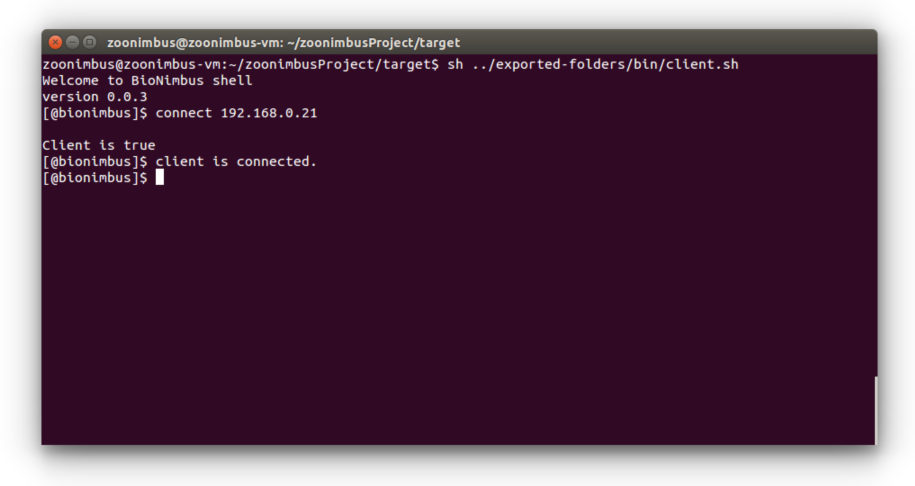
\includegraphics[scale=0.49]{terminal_bionimbuz.png}
	\caption{\textit{Terminal} do BioNimbuZ.}
	\label{fig:terminal_bionimbuz}
\end{figure}

Dessa forma, utilizando a interface mostrada na Figura \ref{fig:terminal_bionimbuz}, para o usuário submeter um \textit{workflow} com dois passos, a seguinte sequência de comandos deveria ser executada:

\begin{enumerate}
	\item [1.] Executar o comando \textbf{\textit{connect}} para se conectar ao BioNimbuZ, passando o IP da máquina servidora como argumento do comando;
    \item [2.] Enviar cada arquivo a partir do comando \textbf{\textit{upload}}, passando o caminho do arquivo à ser enviado;
    \item [3.] Com todos os arquivos enviados, submeter o comando \textbf{\textit{start}} passando o identificador do primeiro serviço (nesse caso, serviço se refere ao software computacional a ser executado naquele \textit{job} e uma lista contendo os serviços disponíveis era mostrada a partir do comando \textbf{\textit{services}}), a lista de arquivos de entrada e a lista de arquivos de saída;
    \item [4.] A partir do início de um \textit{job} era possível verificar seu \textit{status} com o comando \textbf{\textit{status}}, informando o número do \textit{job}.
\end{enumerate}

Os comandos acima descrevem o passo a passo da execução de apenas um \textit{job}. Para um segundo passo, seria necessário submeter todos esses comandos novamente, com os dados de entrada do segundo \textit{job}. Assim, o método acima, via \textit{terminal}, não dava suporte à execução de \textit{workflows}, pois não era possível ligar elementos, formar dependências e controlar o fluxo de dados de maneira única. Eram necessárias diversas iterações da sequência de comandos acima descrita para se ter uma ligação entre os \textit{jobs} que o usuário quisesse executar. Dessa forma, o usuário deveria ter informações que, nem sempre, eram de seu conhecimento, como o \textit{IP} da máquina servidora do BioNimbuZ, o caminho do arquivo ou os argumentos de um serviço provido. 

Portanto, tendo como base [], que diz que o ciclo de vida de um \textit{workflow} é composto pelos passos de projeto e composição, planejamento de recursos, execução, análise e compartilhamento de resultados, foi verificado que o acesso aos serviços providos pelo BioNimbuZ via \textit{terminal} poderia ser melhorado caso alguns requisitos fossem implementados, tais como:

\begin{itemize}
	\item \textbf{Acesso via \textit{Internet}:} Prover de um meio de acesso à plataforma do BioNimbuZ à qualquer pessoa conectada à \textit{Internet};
    \item \textbf{Composição do \textit{workflow} de maneira gráfica:} Um \textit{workflow} científico é composto por uma sequência de passos interligados, formando uma cadeia de execução com entradas e saídas. A forma mais viável de projetá-lo seria a partir de uma interface que possibilitasse o desenho de um \textit{workflow};
	\item \textbf{Acesso à plataforma utilizando-se usuário e senha:} O acesso via \textit{terminal} não dava suporte à múltiplos usuários. Cada usuário deveria ter o BioNimbuZ instalado em seu computador e submetia sua sequência de \textit{jobs} da sua máquina para o servidor do BioNimbuZ. Assim, por questões de segurança, fez-se necessário o desenvolvimento de um método de controle de usuários, verificando a autenticidade e a autorização no momento do \textit{login};
    \item \textbf{Facilidade no envio dos arquivos:} O método de envio dos arquivos poderia ser facilitado, caso fosse desenvolvido uma maneira gráfica de enviá-los ao BioNimbuZ;
    \item \textbf{Controle do \textit{status} dos \textit{workflows} submetidos:} Método de visualização do \textit{status} de cada \textit{workflow} que o submeteu para ser processado pela plataforma do BioNimbuZ.
    \item \textbf{Separação entre aplicação cliente e aplicação servidora:} Evitaria um ponto único de falhas, pois as aplicações poderiam ser executadas em ambientes diferentes, em infraestruturas diferentes e, no caso de falha de uma delas, a outra não seria prejudicada. Com esse requisito também seria possível reduzir custos, pois a infraestrutura necessária para executar a aplicação cliente não tem a necessidade de ser tão robusta quanto a aplicação servidora, pois apenas esta executaria os serviços computacionais providos pelo BioNimbuZ.
\end{itemize}

Na próxima Seção, será apresentada a nova arquitetura, contendo requisitos descritos acima que possibilitaram o desenvolvimento do Sistema Gerenciador de \textit{Workflows} Científicos, objetivo deste trabalho.

\section{Proposta de uma Nova Arquitetura} \label{cap5sec2}

Tendo em vista os requisitos levantados, descritos na Seção \ref{cap5sec1}, e para que o BioNimbuZ se tornasse acessível através da Internet, foi necessário a implementação de um método de acesso baseado em tecnologias \textit{web}, substituindo o método antigo via \textit{terminal}. Para isso, foi desenvolvida um sistema gerenciador de \textit{workflows} basado em interface gráfica utilizando a linguagem de programação Java, em conjunto com \textit{frameworks web}. Para tal, uma nova proposta de arquitetura foi concebida, englobando as modificações necessárias (principalmente, na parte de comunicação entre os seguintes componentes do sistema: Aplicação \textit{Web} e Núcleo). 

Nessa nova arquitetura, o BioNimbuZ não será composto apenas pelas três camadas projetadas anteriormente [3] (Aplicação, Núcleo e Infraestrutura). Será acrescentado um novo componente chamado Camada de Comunicação, devido à importância para a troca de mensagens entre a aplicação \textit{web} e o núcleo do BioNimbuZ nessa nova abordagem. Assim, a Figura \ref{fig:proposta_arquitetura} apresenta ess nova proposta de arquitetura e uma breve descrição dos componentes (sua explicação completa será apresentada na próxima Seção, \ref{cap5sec3}): 

\begin{figure}[H]
	\centering
	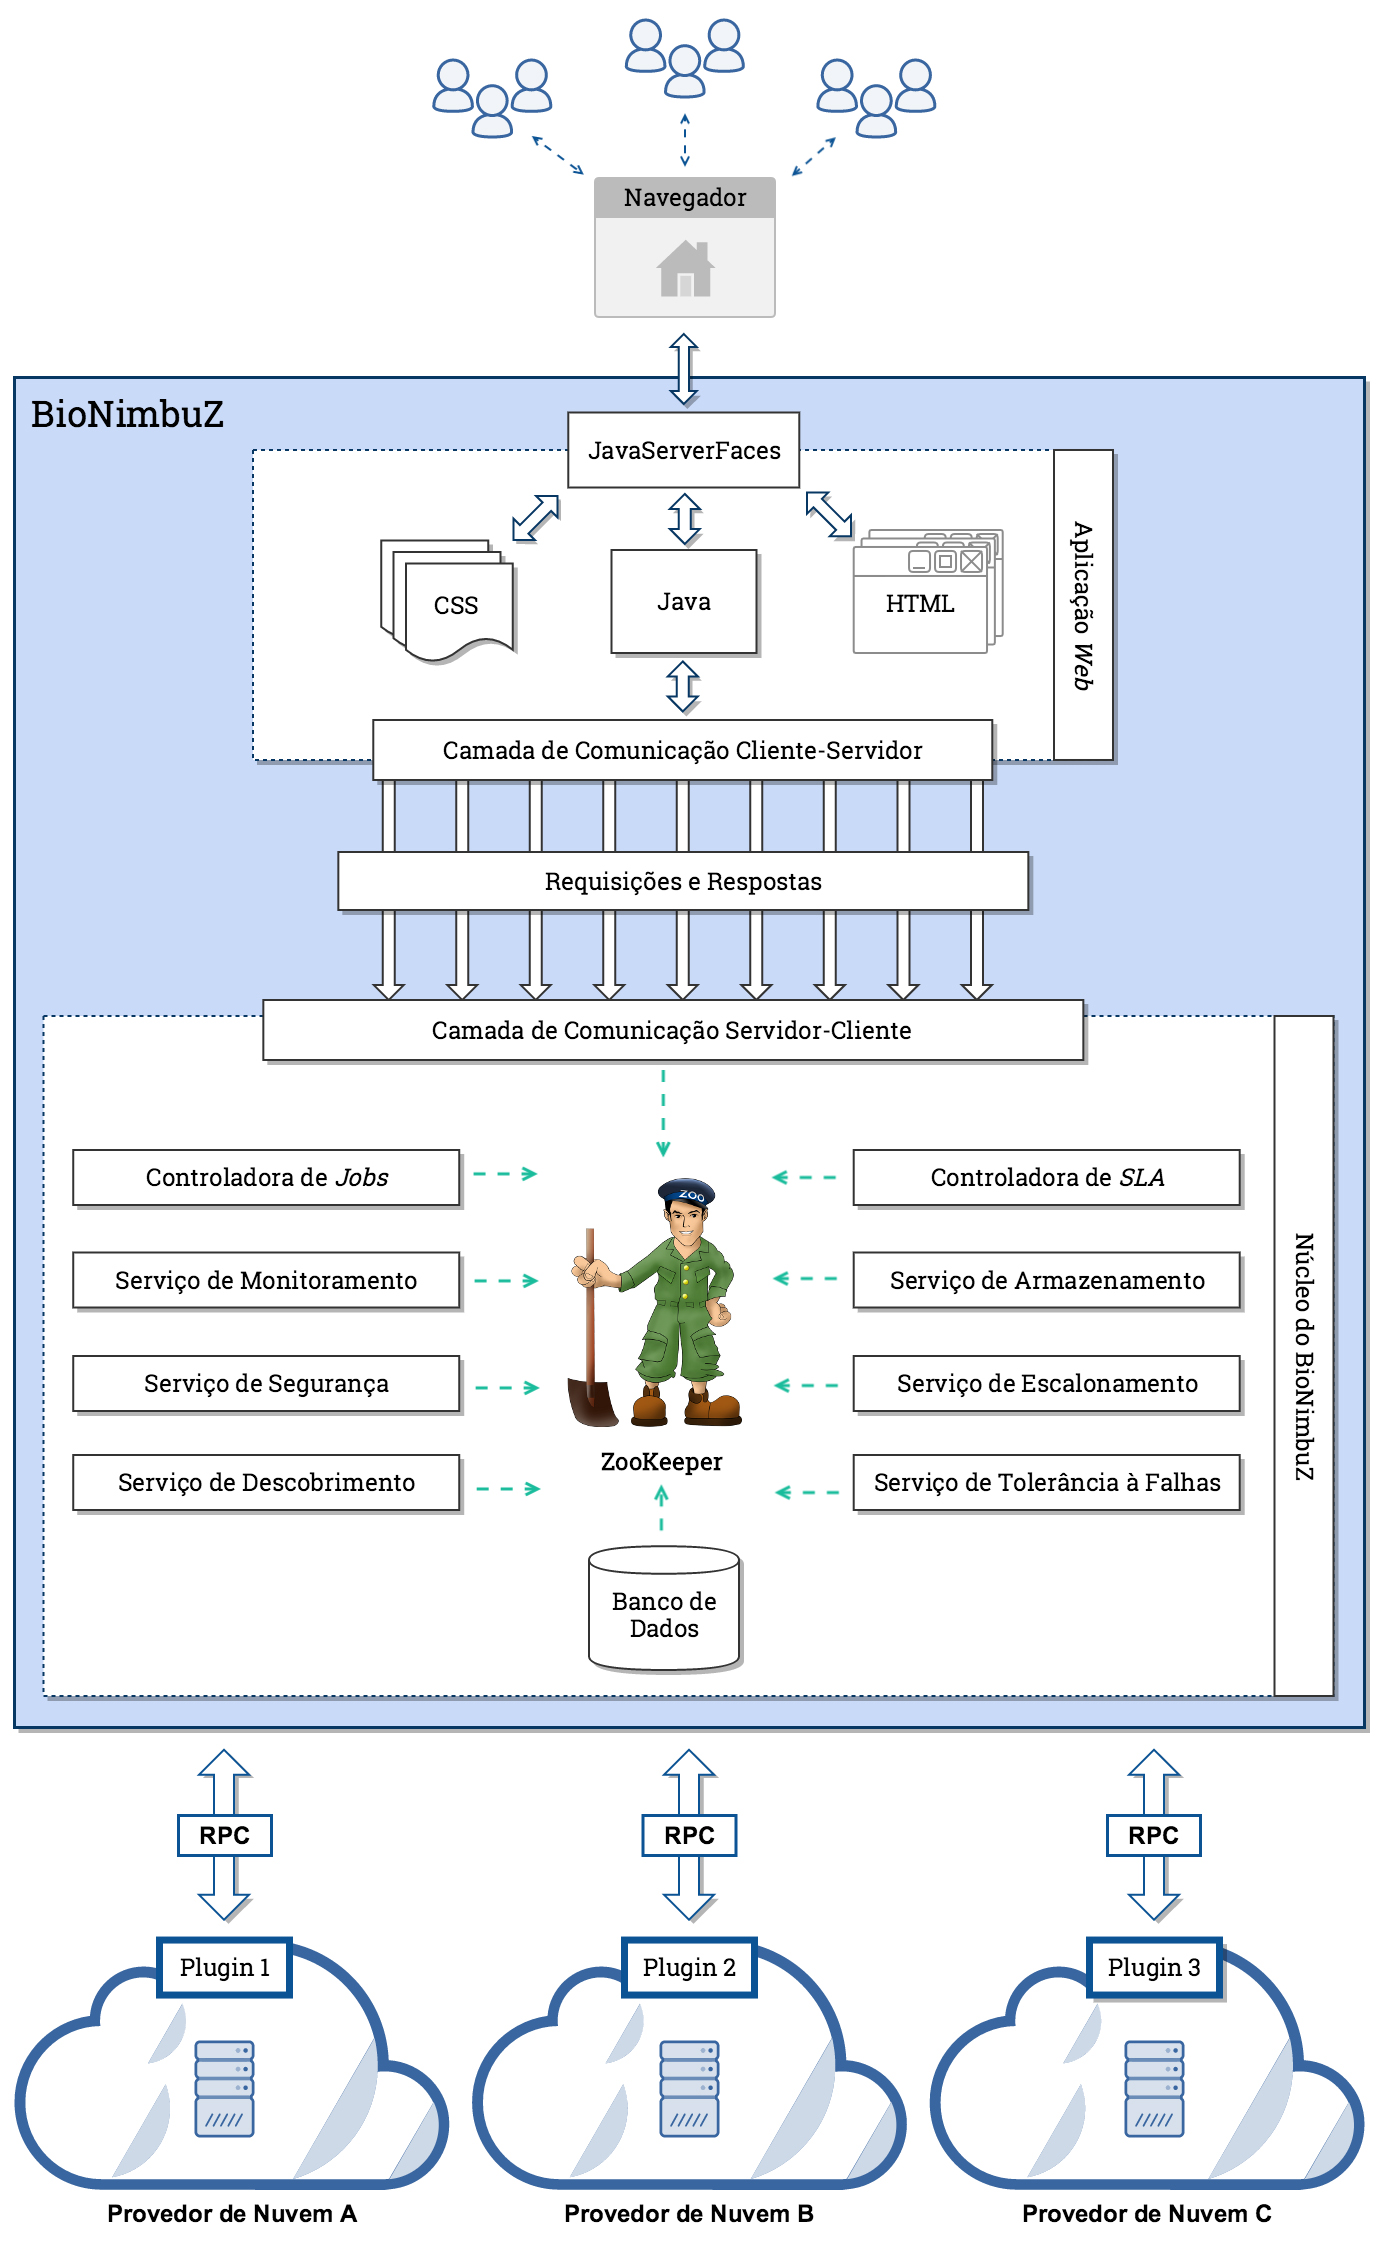
\includegraphics[scale=0.27 ]{nova_arquitetura.jpg}
	\caption{Nova Arquitetura do BioNimbuZ.}
	\label{fig:proposta_arquitetura}
\end{figure}

\begin{itemize}
	\item \textbf{Aplicação \textit{Web}:} Implementa o sistema gerenciador de \textit{workflows} científicos e utiliza a camada de comunicação para enviar requisições e receber respostas do núcleo.
    \item \textbf{Camada de Comunicação:} Implementa a troca de mensagens entre o núcleo e a aplicação \textit{web} utilizando \textit{webservices}, disparando requisições da aplicação \textit{web} para o núcleo e recebendo respostas do núcleo para a aplicação.
    \item \textbf{Núcleo:} Responsável pelo armazenamento de arquivos, escalonamento de \textit{jobs}, execução de \textit{workflows}, acesso ao banco de dados, descobrimento dos provedores e o gerenciamento de possíveis falhas.

\item \textbf{Infraestrutura:} Composta pelos provedores de serviço utilizados pelo BioNimbuZ e que compõem sua federação de nuvens.
\end{itemize}

As Seções \ref{cap5sec3}, \ref{cap5sec4} e \ref{cap5sec5} trazem detalhes das camadas supracitadas.

\section{Aplicação \textit{Web}} \label{cap5sec3}
%	Para que o BioNimbuZ se tornasse acessível através da Internet, foi necessária a implementação de um método de acesso baseado em tecnologias Web. Para isso, foi desenvolvida um Sistema Gerenciador de \textit{Workflows} basado em interface gráfica utilizando a linguagem de programação Java, em conjunto com outros \textit{frameworks}, como: Java JSF, biblioteca de componentes visuais PrimeFaces, páginas HTML, códigos de estilo CSS.
    
	Este componente compreende o Sistema Gerenciador de \textit{Workflows} Científicos e deve prover meios para que usuários possam se logar no sistema BioNimbuZ através de uma interface gráfica acessível pela Internet e utilizem suas funcionalidades como envio de arquivos (que serão utilizados como entrada dos \textit{workflows} criados pelo usuário), exclusão de arquivos, visualização dos dados de saída gerados pela execução de seus \textit{workflows}, por exemplo. Pela interface, o usuário também deve ser capaz de criar e projetar seus \textit{workflows} de maneira gráfica, ligando passos, indicando dependências, incluindo argumentos e indicando quais arquivos de entrada serão utilizados.
    
Com os requisitos descritos na Seção anterior, foi projetada a implementação desse componente através da linguagem de programação Java e \textit{frameworks Web} (bibliotecas de \textit{software} que facilitam a implementação de funcionalidade relacionadas à sistemas voltados para \textit{internet}). 

Na implementação de uma aplicação \textit{Web}, o desenvolvimento é dividido em camadas e utiliza-se, normalmente, o padrão de projeto \textit{MVC} (\textit{Model-View-Controller}) \cite{design_patterns}. O padrão \textit{MVC} é utilizado no desenvolvimento de interfaces pela sua cartacterística de estar intimamente mapeado nos aspectos principais de uma interface: 

\begin{itemize}
	\item \textbf{Visualização:} Fornece a apresentação do dados presentes no Modelo.
    \item \textbf{Controlador:} Recebe os dados e comandos do usuário e determina o que isso significa para o Modelo.
    \item \textbf{Modelo:} Contém todos os dados e estados persistidos, geralmente em Bancos de Dados.
\end{itemize}

Dessa forma, o padrão \textit{MVC} contém exatamente esse três componentes: o \textbf{\textit{Model}} (Modelo), o \textbf{\textit{Controller}} (Controlador) e o \textbf{\textit{View}} (Visualização). A interação entre esses componentes pode ser descrita da seguinte maneira:

\begin{figure}[H]
	\centering
	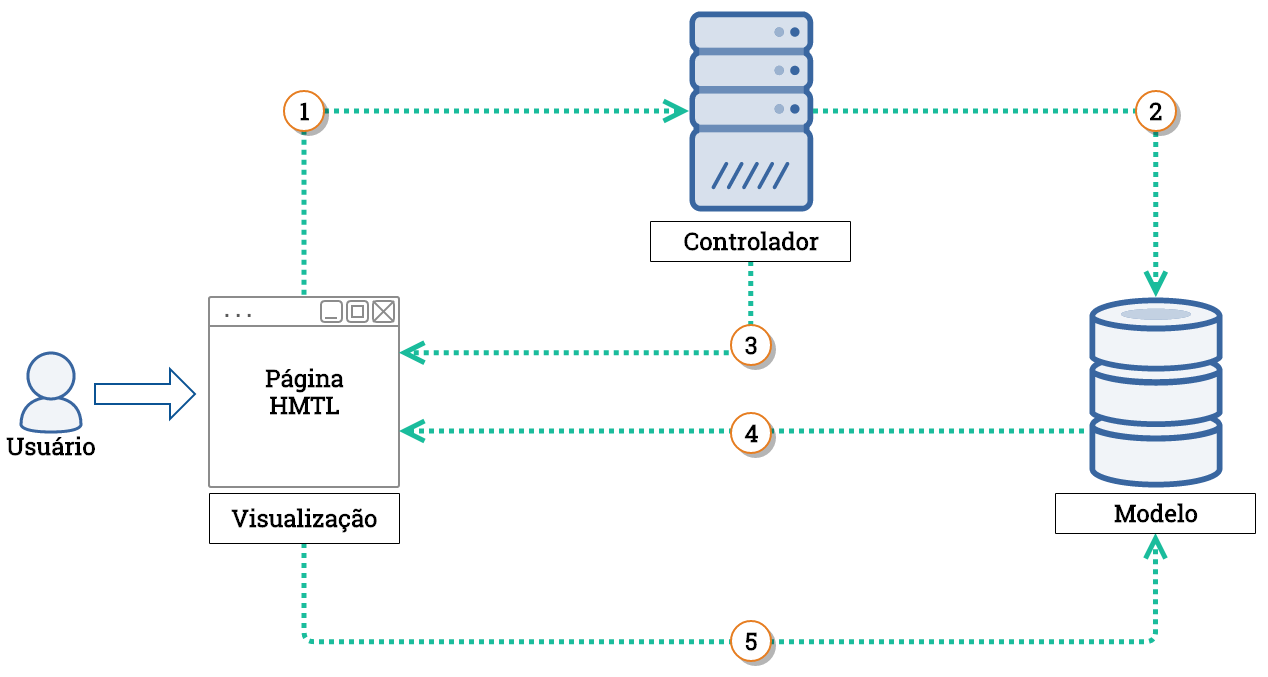
\includegraphics[scale=0.25 ]{padrao_mvc.png}
	\caption{Modelo \textit{Model-View-Controller}.}
	\label{fig:padrao_mvc}
\end{figure}

Na Figura \ref{fig:padrao_mvc}, o fluxo pode ser descrito como se segue:

\begin{itemize}
 	\item \textbf{(1):} O usuário realiza uma ação na página HTML.
    \item \textbf{(2):} O Controlador processa o comando e muda o estado de algum objeto no Modelo.
    \item \textbf{(3):} O Controlador envia um comando à Visualização para modificar os dados exibidos.
    \item \textbf{(4):} O Modelo notifica a Visualização de que os dados foram modificados.
    \item \textbf{(5):} A Visualização envia uma requisição ao Modelo pedindo o estado de algum dado.
\end{itemize}

Nesse contexto, diversos \textit{frameworks} surgiram voltados para o desenvolvimento de aplicações \textit{web}, tais como: \textit{Spring MVC} [41], \textit{Struts} [42], \textit{JSF} (\textit{JavaServerFaces}) [32], \textit{Play} [43], entre outros. Para esse projeto, o \textit{framework} escolhido foi o \textit{JSF}.

O \textit{JavaServerFaces} é uma especificação Java para a construção de interfaces de usuário baseadas em componentes para aplicações \textit{web}. Possui um modelo de programação dirigido a eventos, abstraindo os detalhes da manipulação e organização dos componentes, permitindo que o programador se concentre na lógica da aplicação.

Dessa forma, utilizando-se o padrão MVC descrito anteriormente, foi projetada e implementada a aplicação \textit{web} contendo os componentes necessários para o desenvolvimento do sistema gerenciador de \textit{workflows} científicos. 

\subsection{Camada de Visualização} \label{cap5sec3subsec1}

Primeiramente, foi desenvolvida a camada de visualização do modelo \textit{MVC}. Para tal, foram desenvolvidas páginas em \textbf{HTML} \cite{html_rfc} (\textit{Hypertext Markup Language}) utilizando componentes visuais da biblioteca \textit{Primefaces} \cite{primefaces_url}. O \textit{framework} \textbf{\textit{Primefaces}} possibilita utilizar componentes visuais ricos e de maneira simples, sem se preocupar em ajustar parâmetros visuais ou de programação.

Abaixo, seguem as telas desenvolvidas para realizar a interface com o usuário e que, juntas, representam a camada de visualização da aplicação \textit{web}. \\


\noindent
\textbf{Tela de Login} \\

\noindent
A Figura \ref{fig:tela_login} mostra a tela inicial da aplicação \textit{web} desenvolvida. Nessa tela, o usuário deve entrar com seu usuário e senha cadastrados previamente para ter acesso aos recursos disponíveis no BioNimbuZ.

\begin{figure}[H]
	\centering
	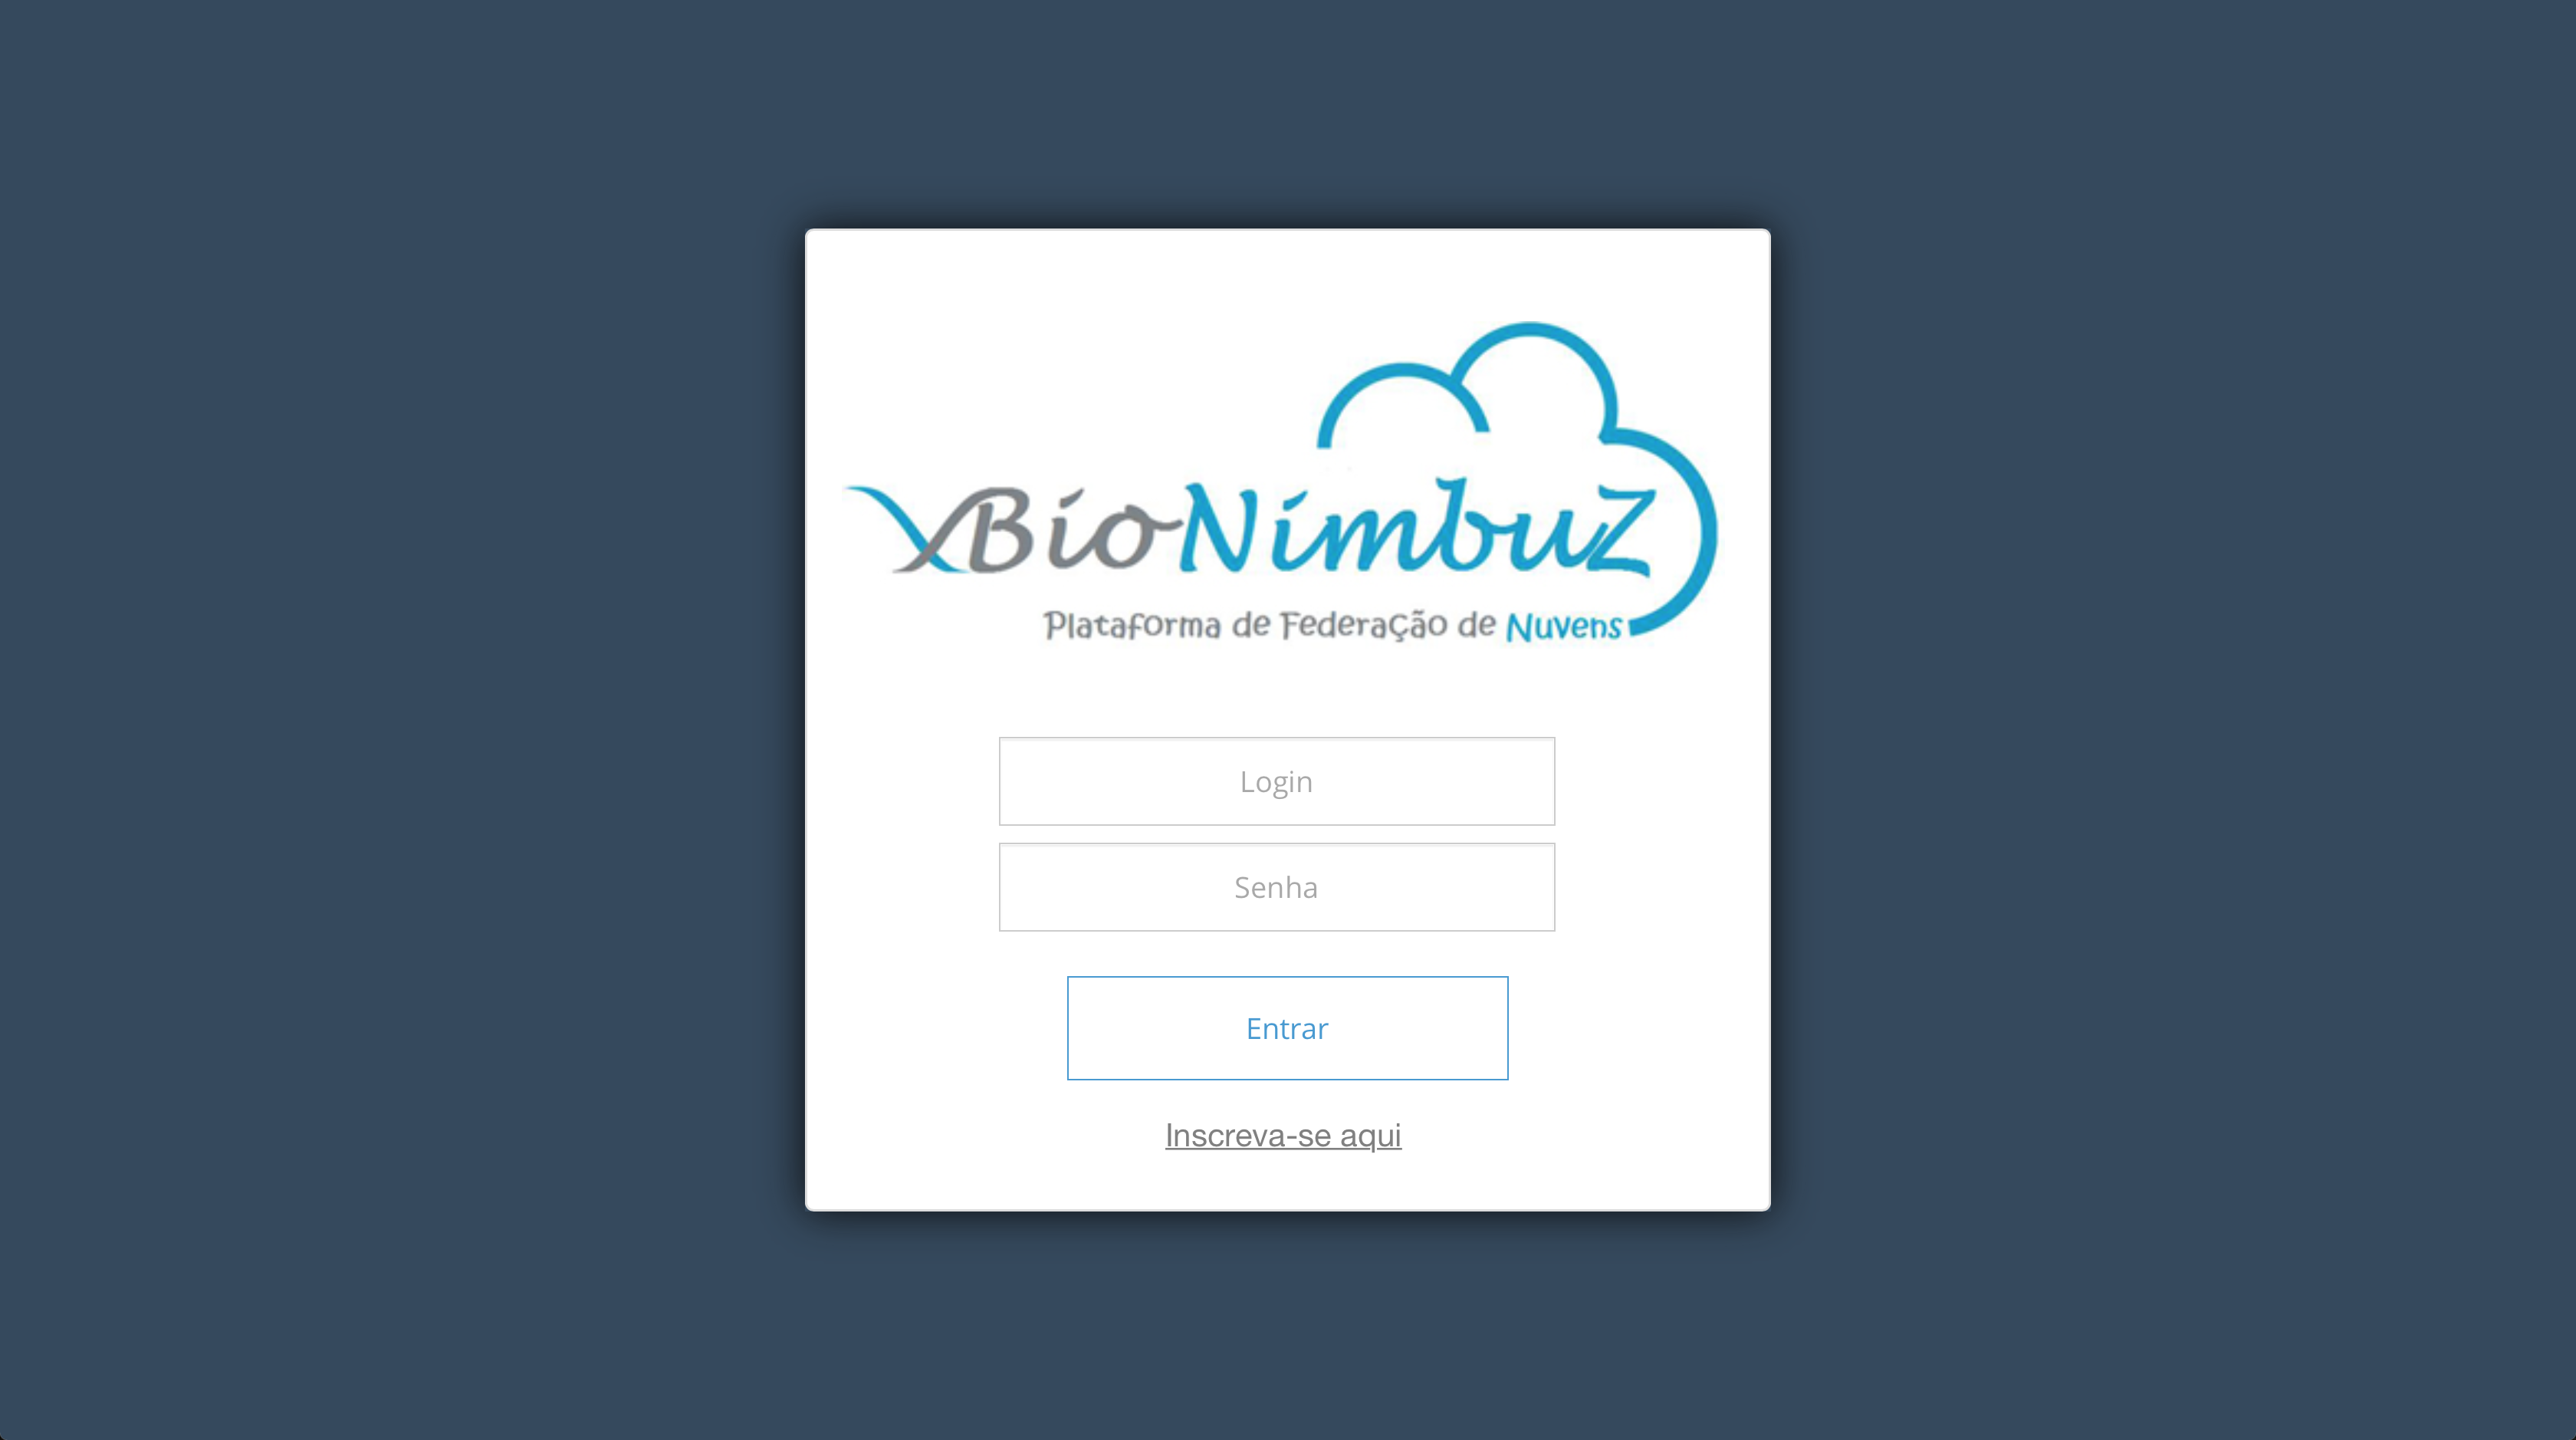
\includegraphics[scale=0.265 ]{tela_login.png}
	\caption{Tela inicial da aplicação \textit{web}.}
	\label{fig:tela_login}
\end{figure}

\noindent
\textbf{Tela de Cadastro} \\

\noindent
Por essa tela, novos usuários se cadastram na plataforma BioNimbuZ, incluindo seus dados, tais como telefone, nome, CPF, etc. A Figura \ref{fig:tela_cadastro} mostra a tela que é apresentada ao usuário.

\begin{figure}[H]
	\centering
	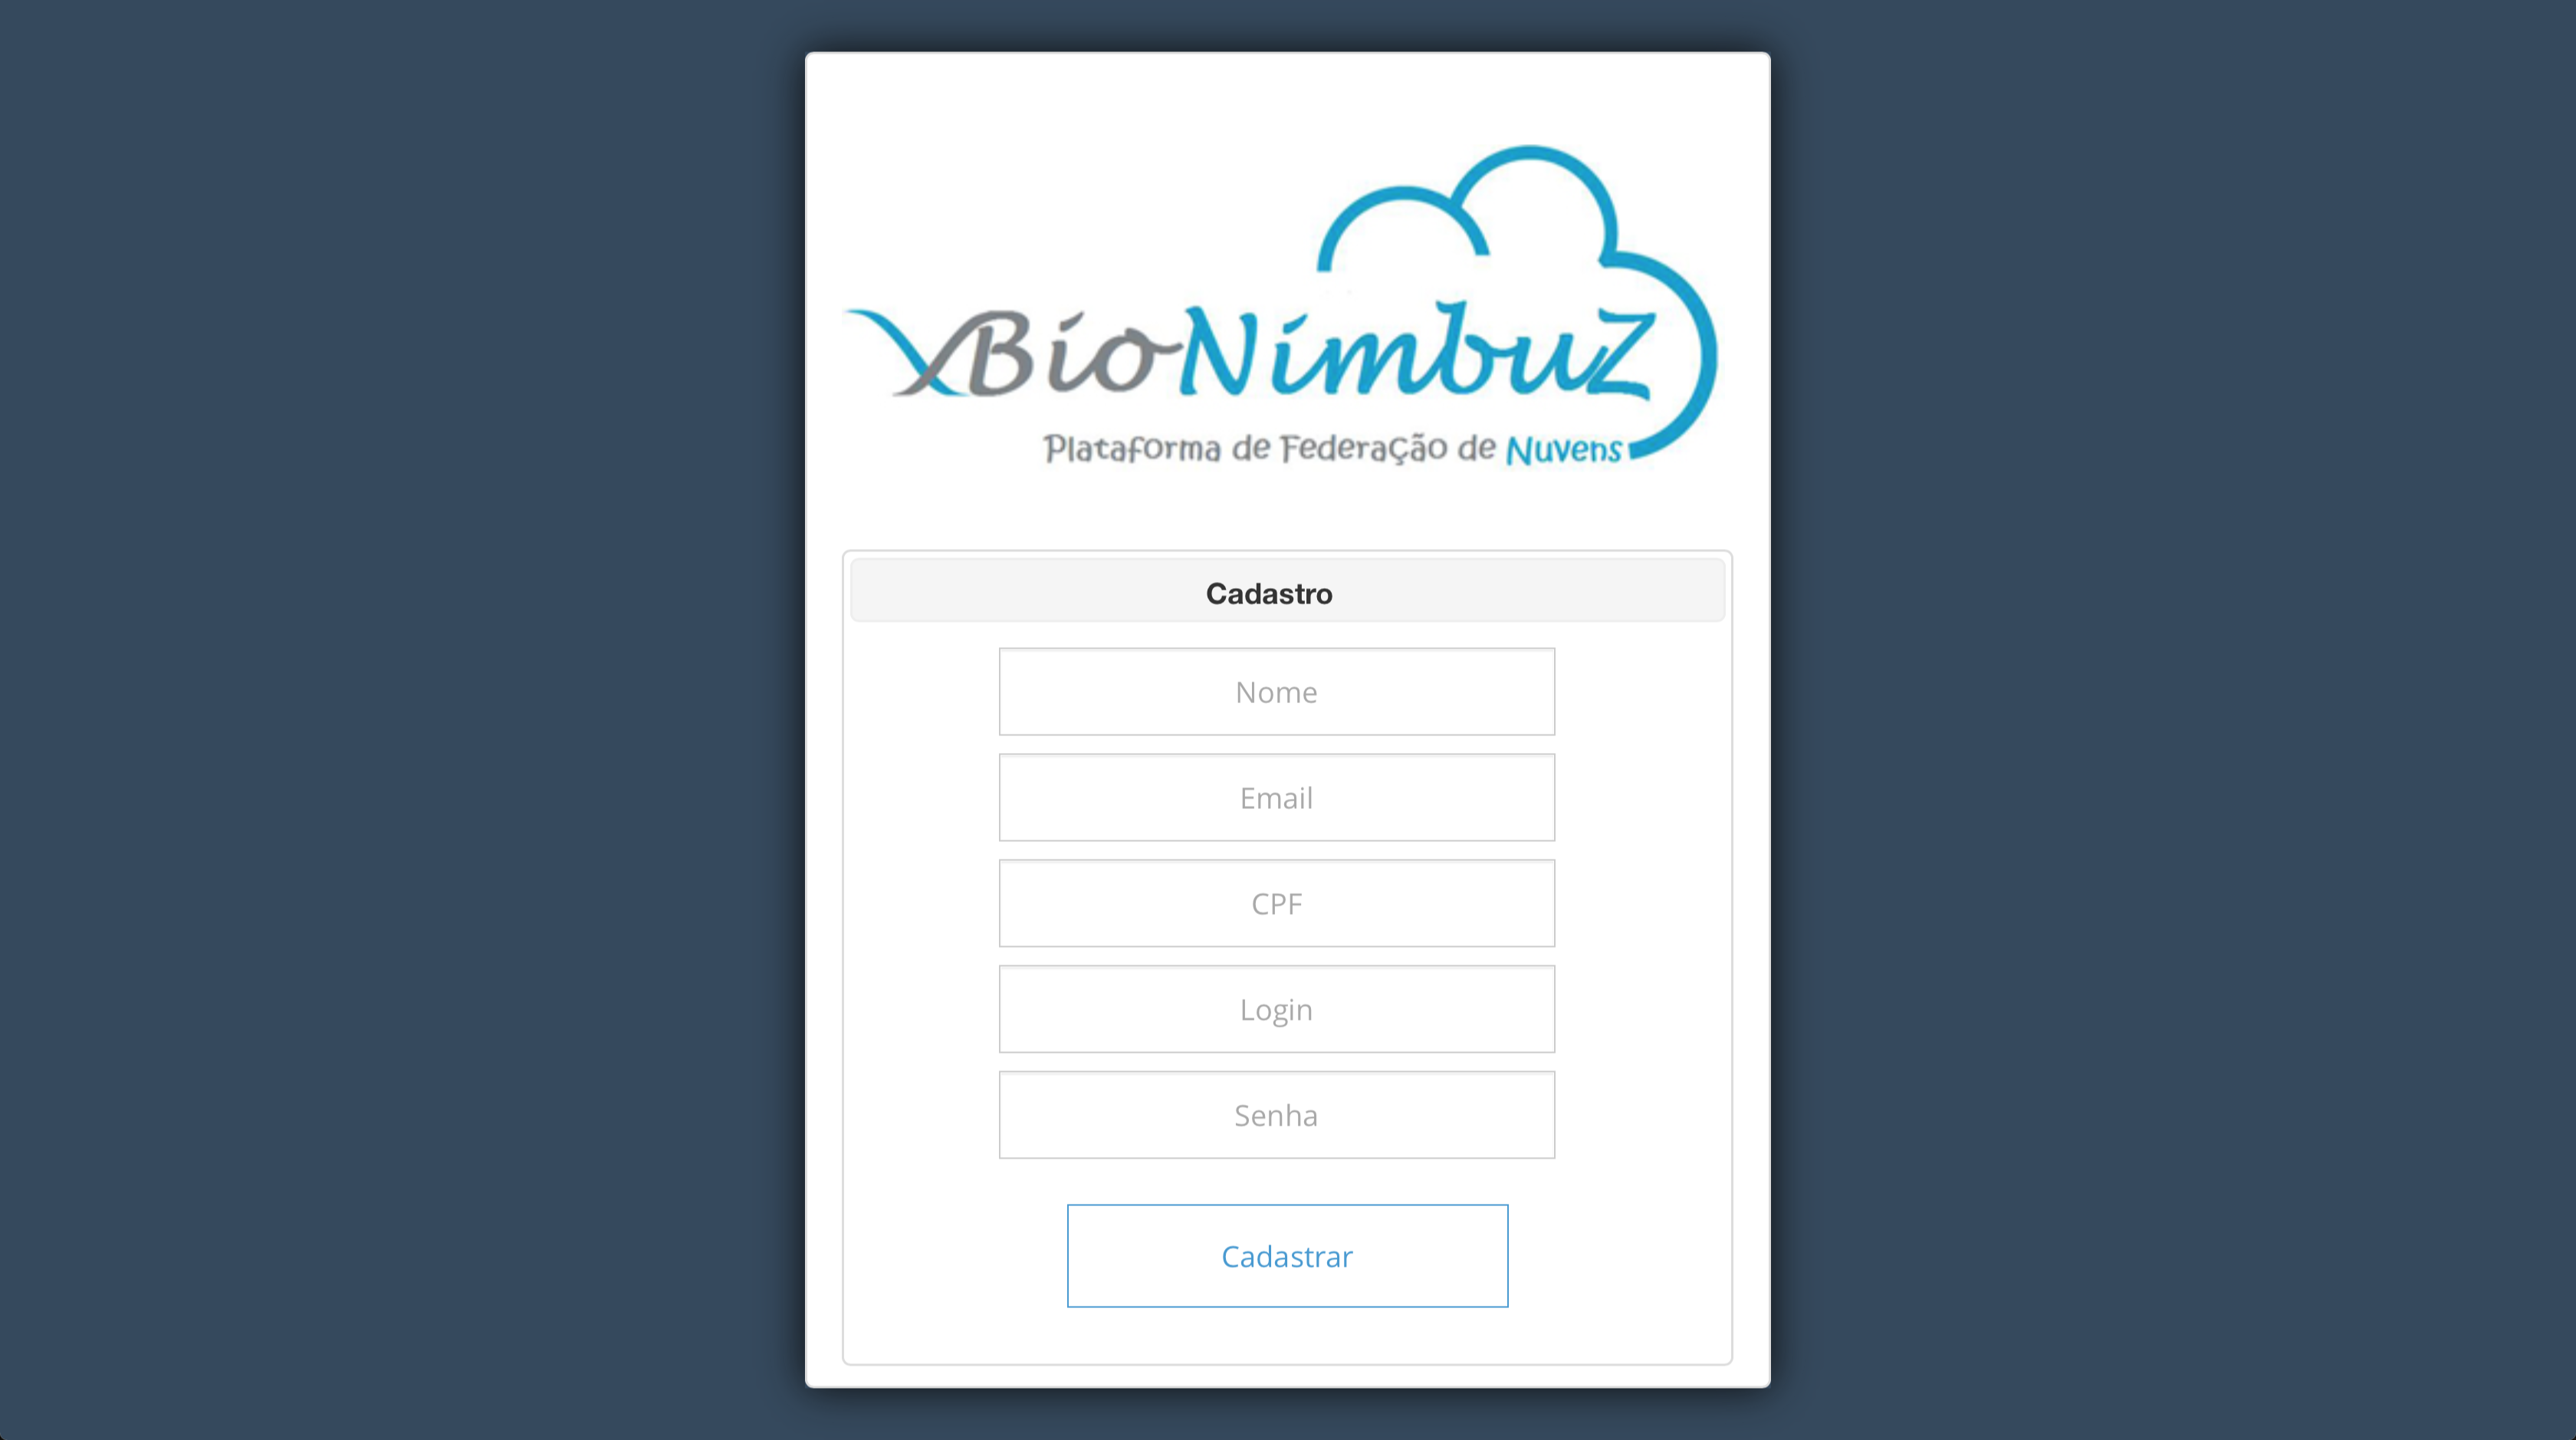
\includegraphics[scale=0.25 ]{tela_cadastro.png}
	\caption{Tela de cadastro de novos usuários.}
	\label{fig:tela_cadastro}
\end{figure}

\noindent
\textbf{\textit{Tela Inicial}} \\

\noindent
Ao realizarem o \textit{login}, os usuários que possuírem acesso ao ambiente \textit{web} visualizarão a tela mostrada na Figura \ref{fig:tela_inicial}. Essa tela dá acesso às opções disponíveis no BioNimbuZ, tais como criar um novo \textit{workflow}, visualizar seu \textit{status}, enviar arquivos para plataforma, etc.

\begin{figure}[H]
	\centering
	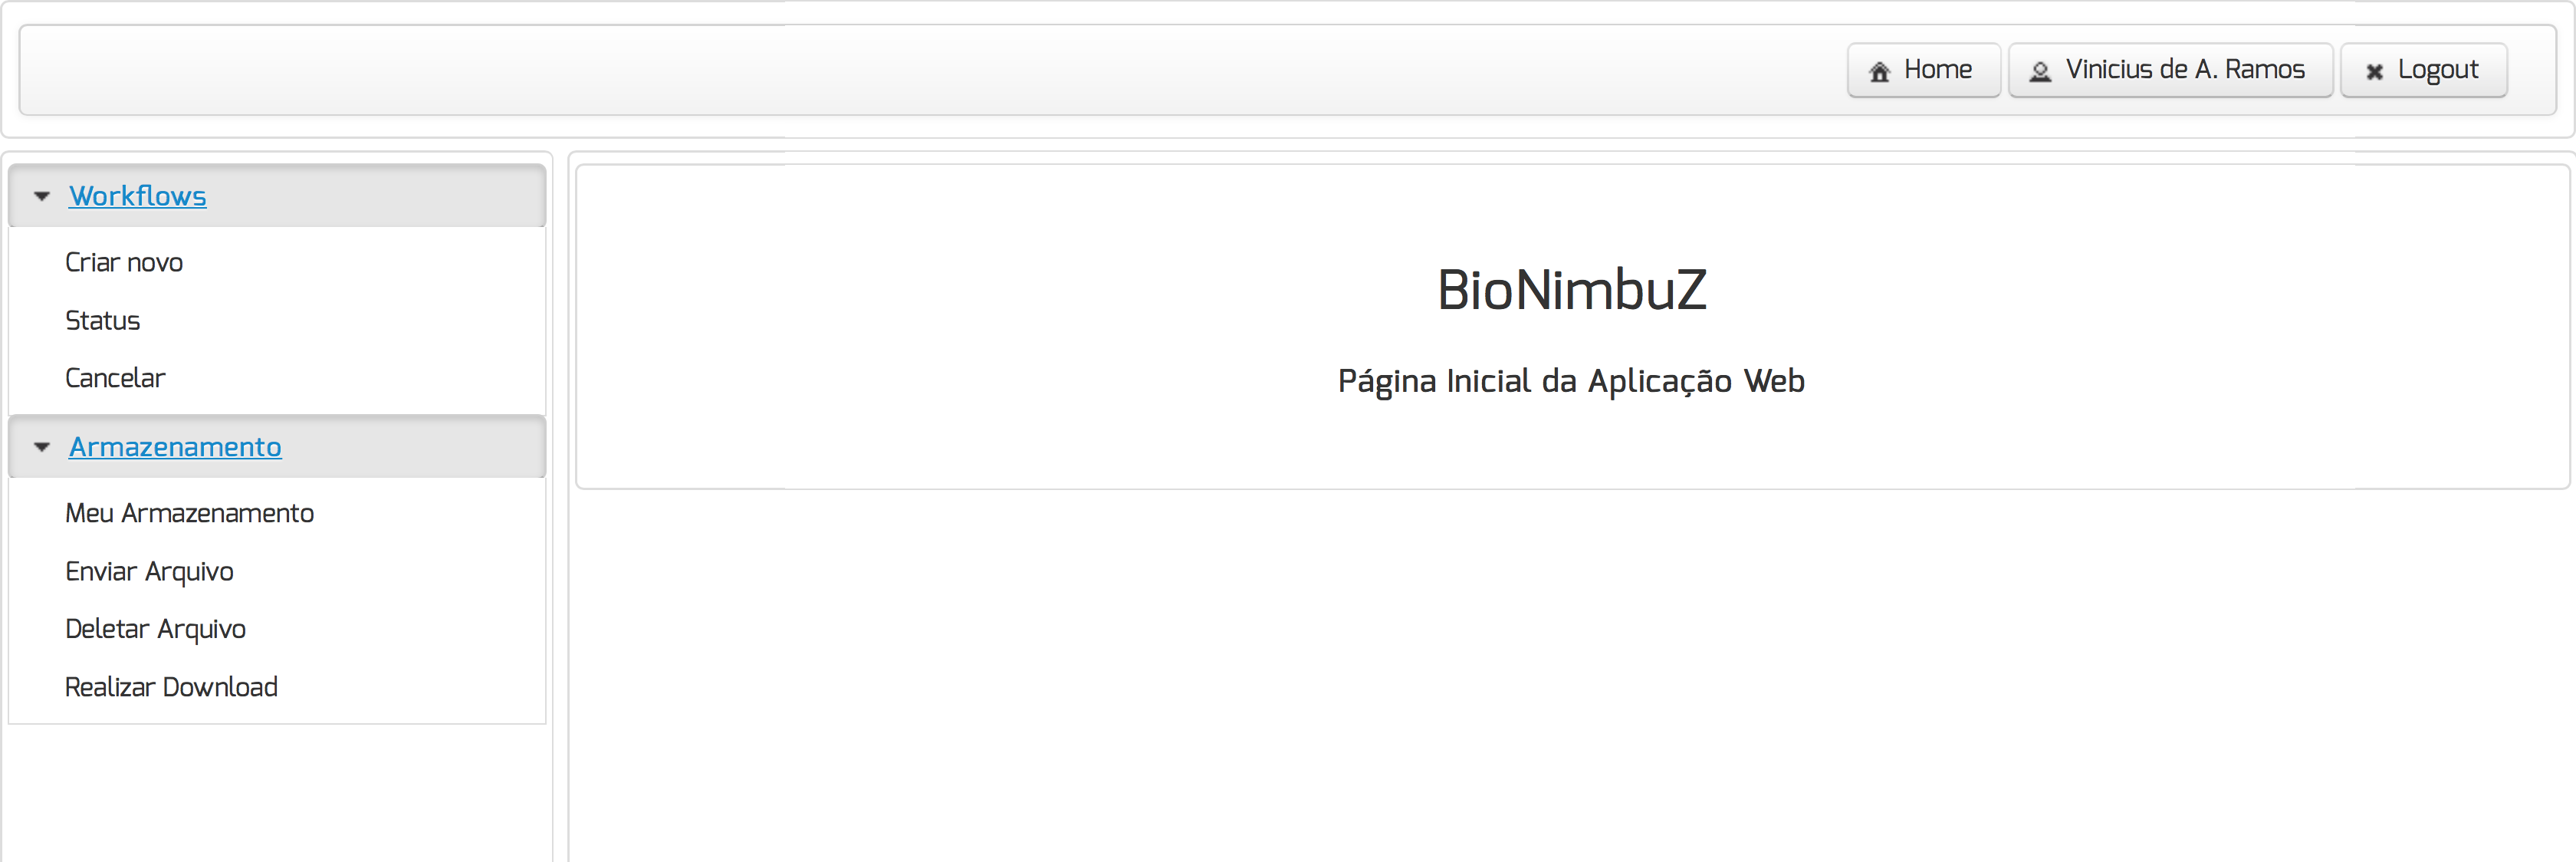
\includegraphics[scale=0.25 ]{tela_inicial.png}
	\caption{Tela inicial da aplicação \textit{web}.}
	\label{fig:tela_inicial}
\end{figure}

\noindent
\textbf{Tela inicial da criação dos \textit{Workflows}} \\

\noindent
Nesta tela, mostrada na Figura \ref{fig:tela_inicial_workflows}, o usuário inicia o projeto de seu \textit{workflow}, podendo escolher entre criar um novo \textit{workflow} ou importar um anteriormente criado. A aplicação \textit{web} possibilita, ao fim do projeto de um \textit{workflow}, exportá-lo. Assim, com esse \textit{workflow} exportado, é possível compartilhá-lo, sendo este a última fase do ciclo de vida de um \textit{workflow} (detalhado no \refCap{capitulo3}).

\begin{figure}[H]
	\centering
	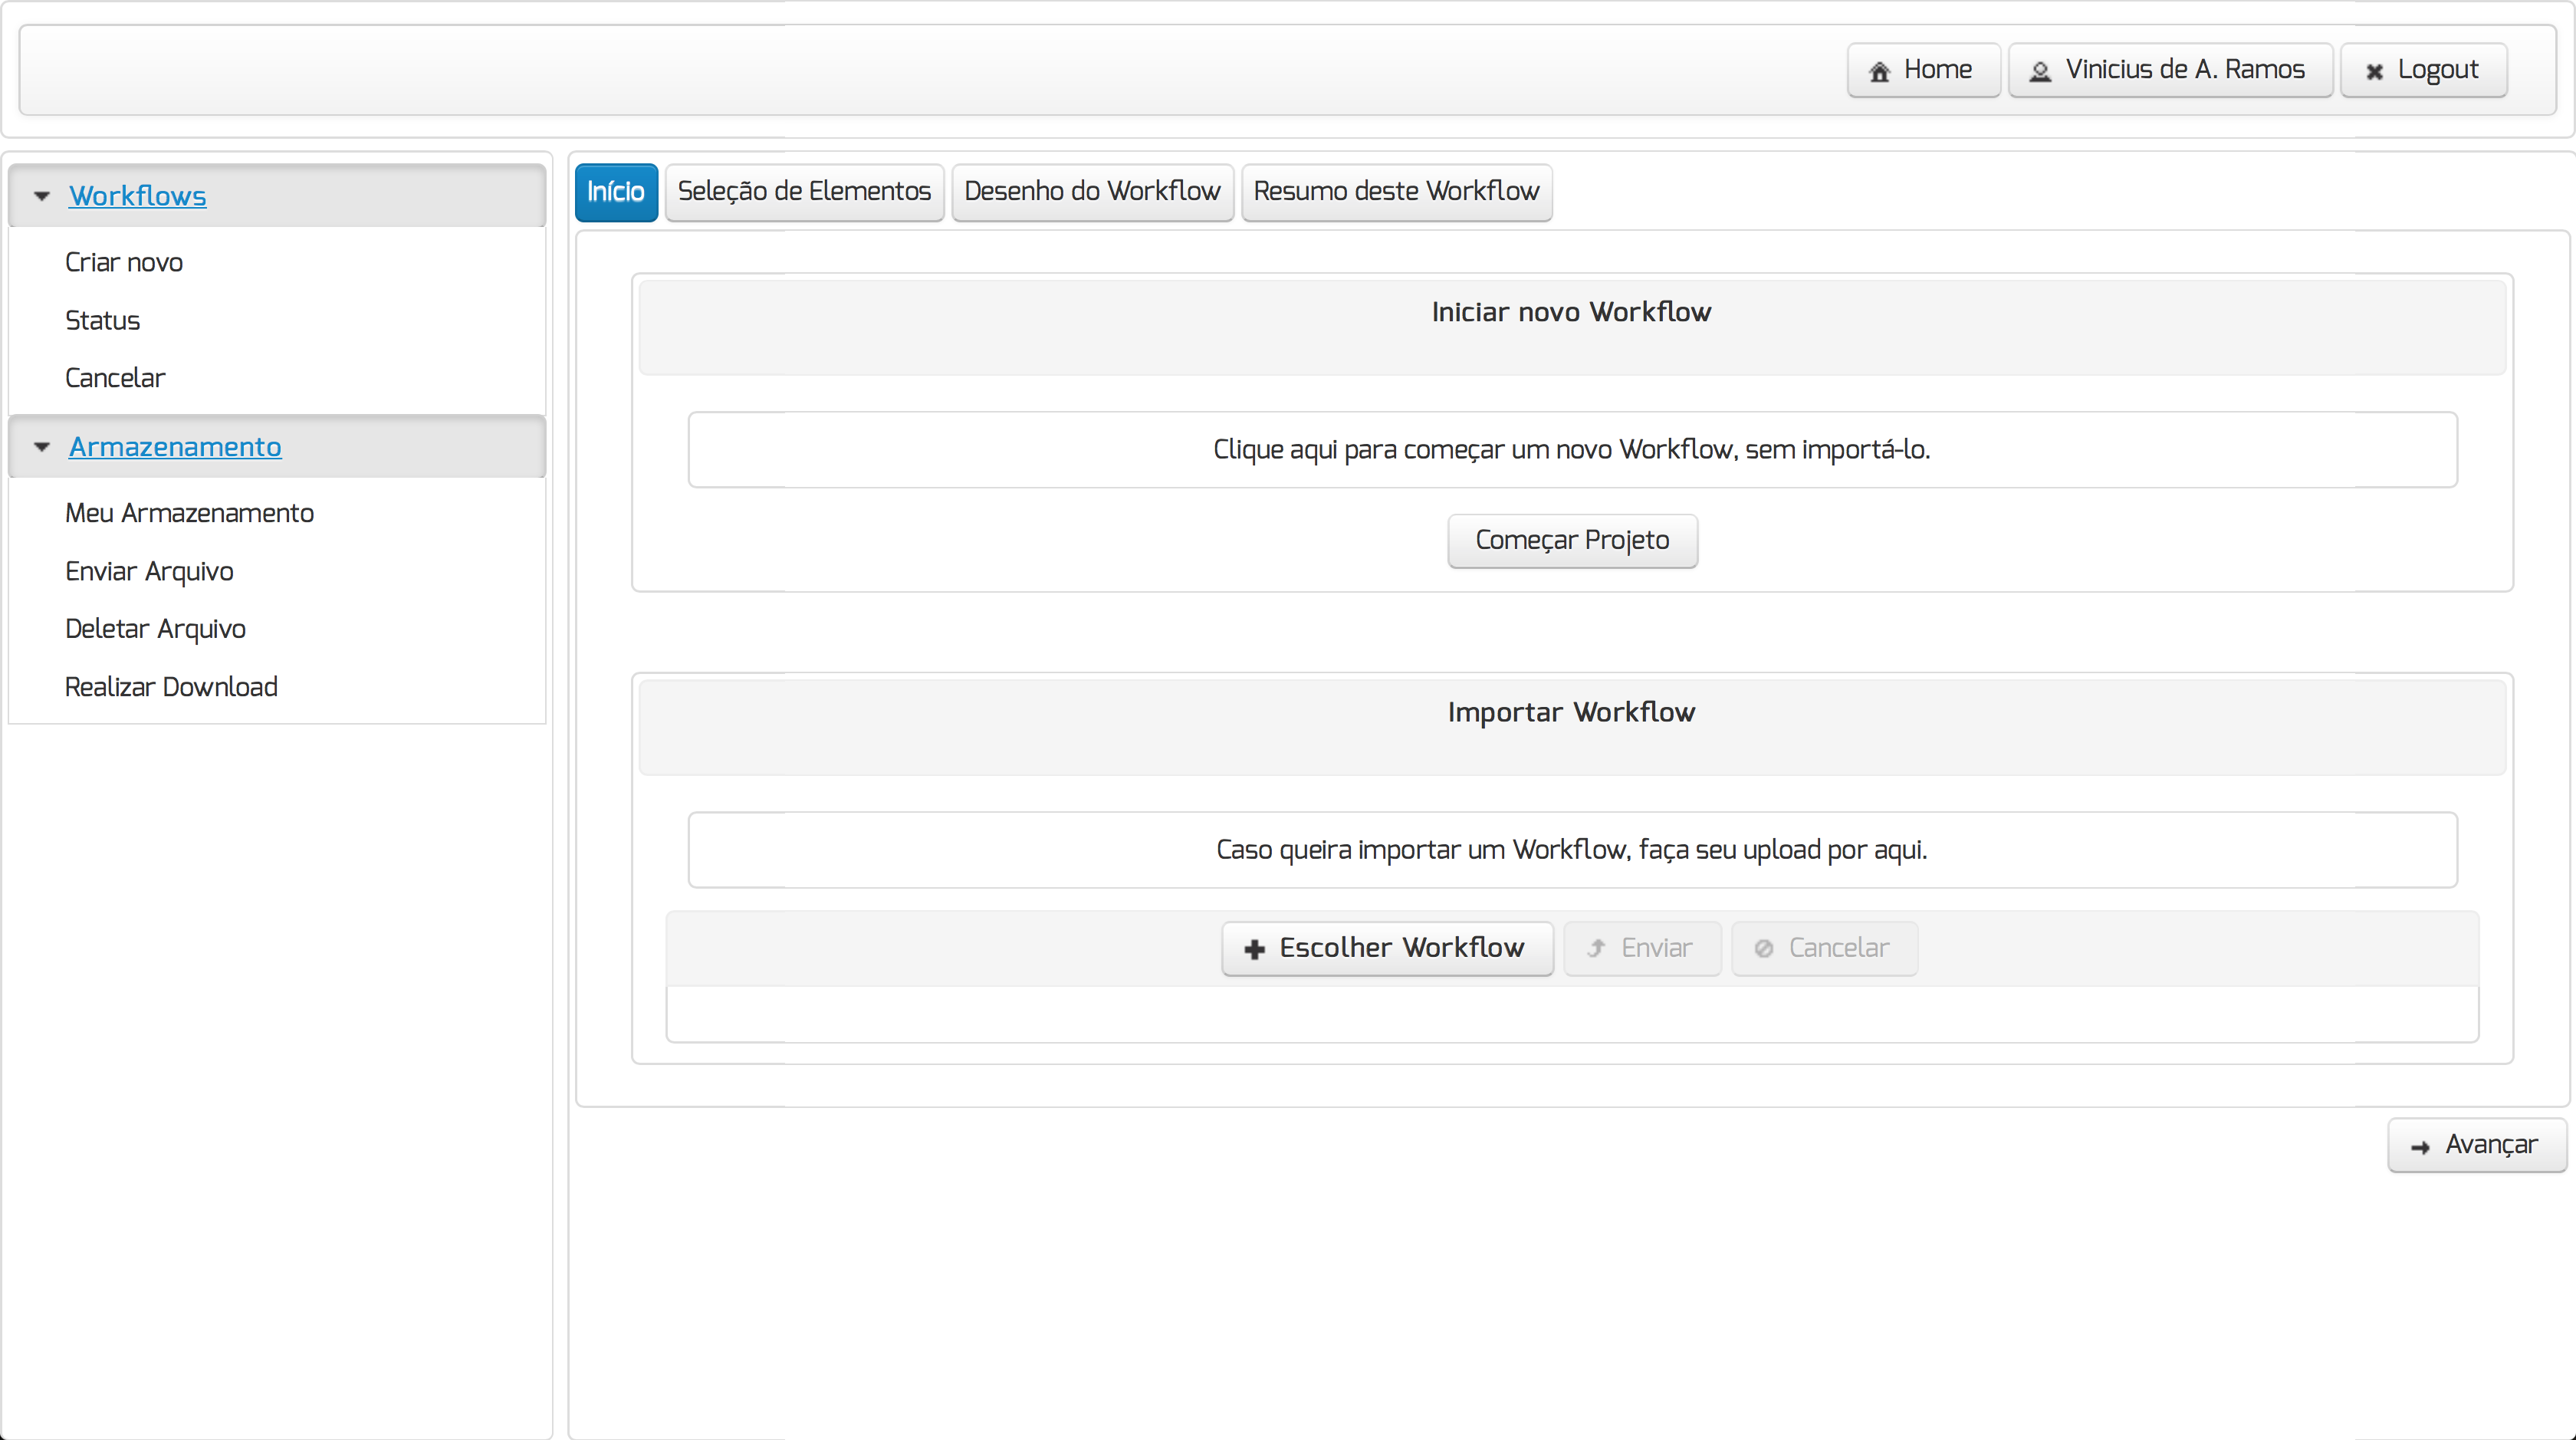
\includegraphics[scale=0.265 ]{tela_inicial_workflows.png}
	\caption{Tela inicial de criação dos \textit{workflows}.}
	\label{fig:tela_inicial_workflows}
\end{figure}

\noindent
\textbf{Tela de seleção de elementos} \\

\noindent
Ao clicar em ''Começar Projeto'', o usuário então é direcionado para a página de seleção de elementos, mostrada na Figura \ref{fig:tela_selecao_elementos}. Nela, o mesmo poderá planejar a execução de seu \textit{workflow}, escolhendo quais elementos irão compor este fluxo. A lista de elementos disponíveis é mantida no núcleo do BioNimbuZ e é enviada à aplicação quando esta é iniciada. À medida que o usuário escolhe os elementos, eles são adicionados na listagem ''Elementos Escolhidos'', podendo o mesmo excluí-los, caso não os queira mais.

\begin{figure}[H]
	\centering
	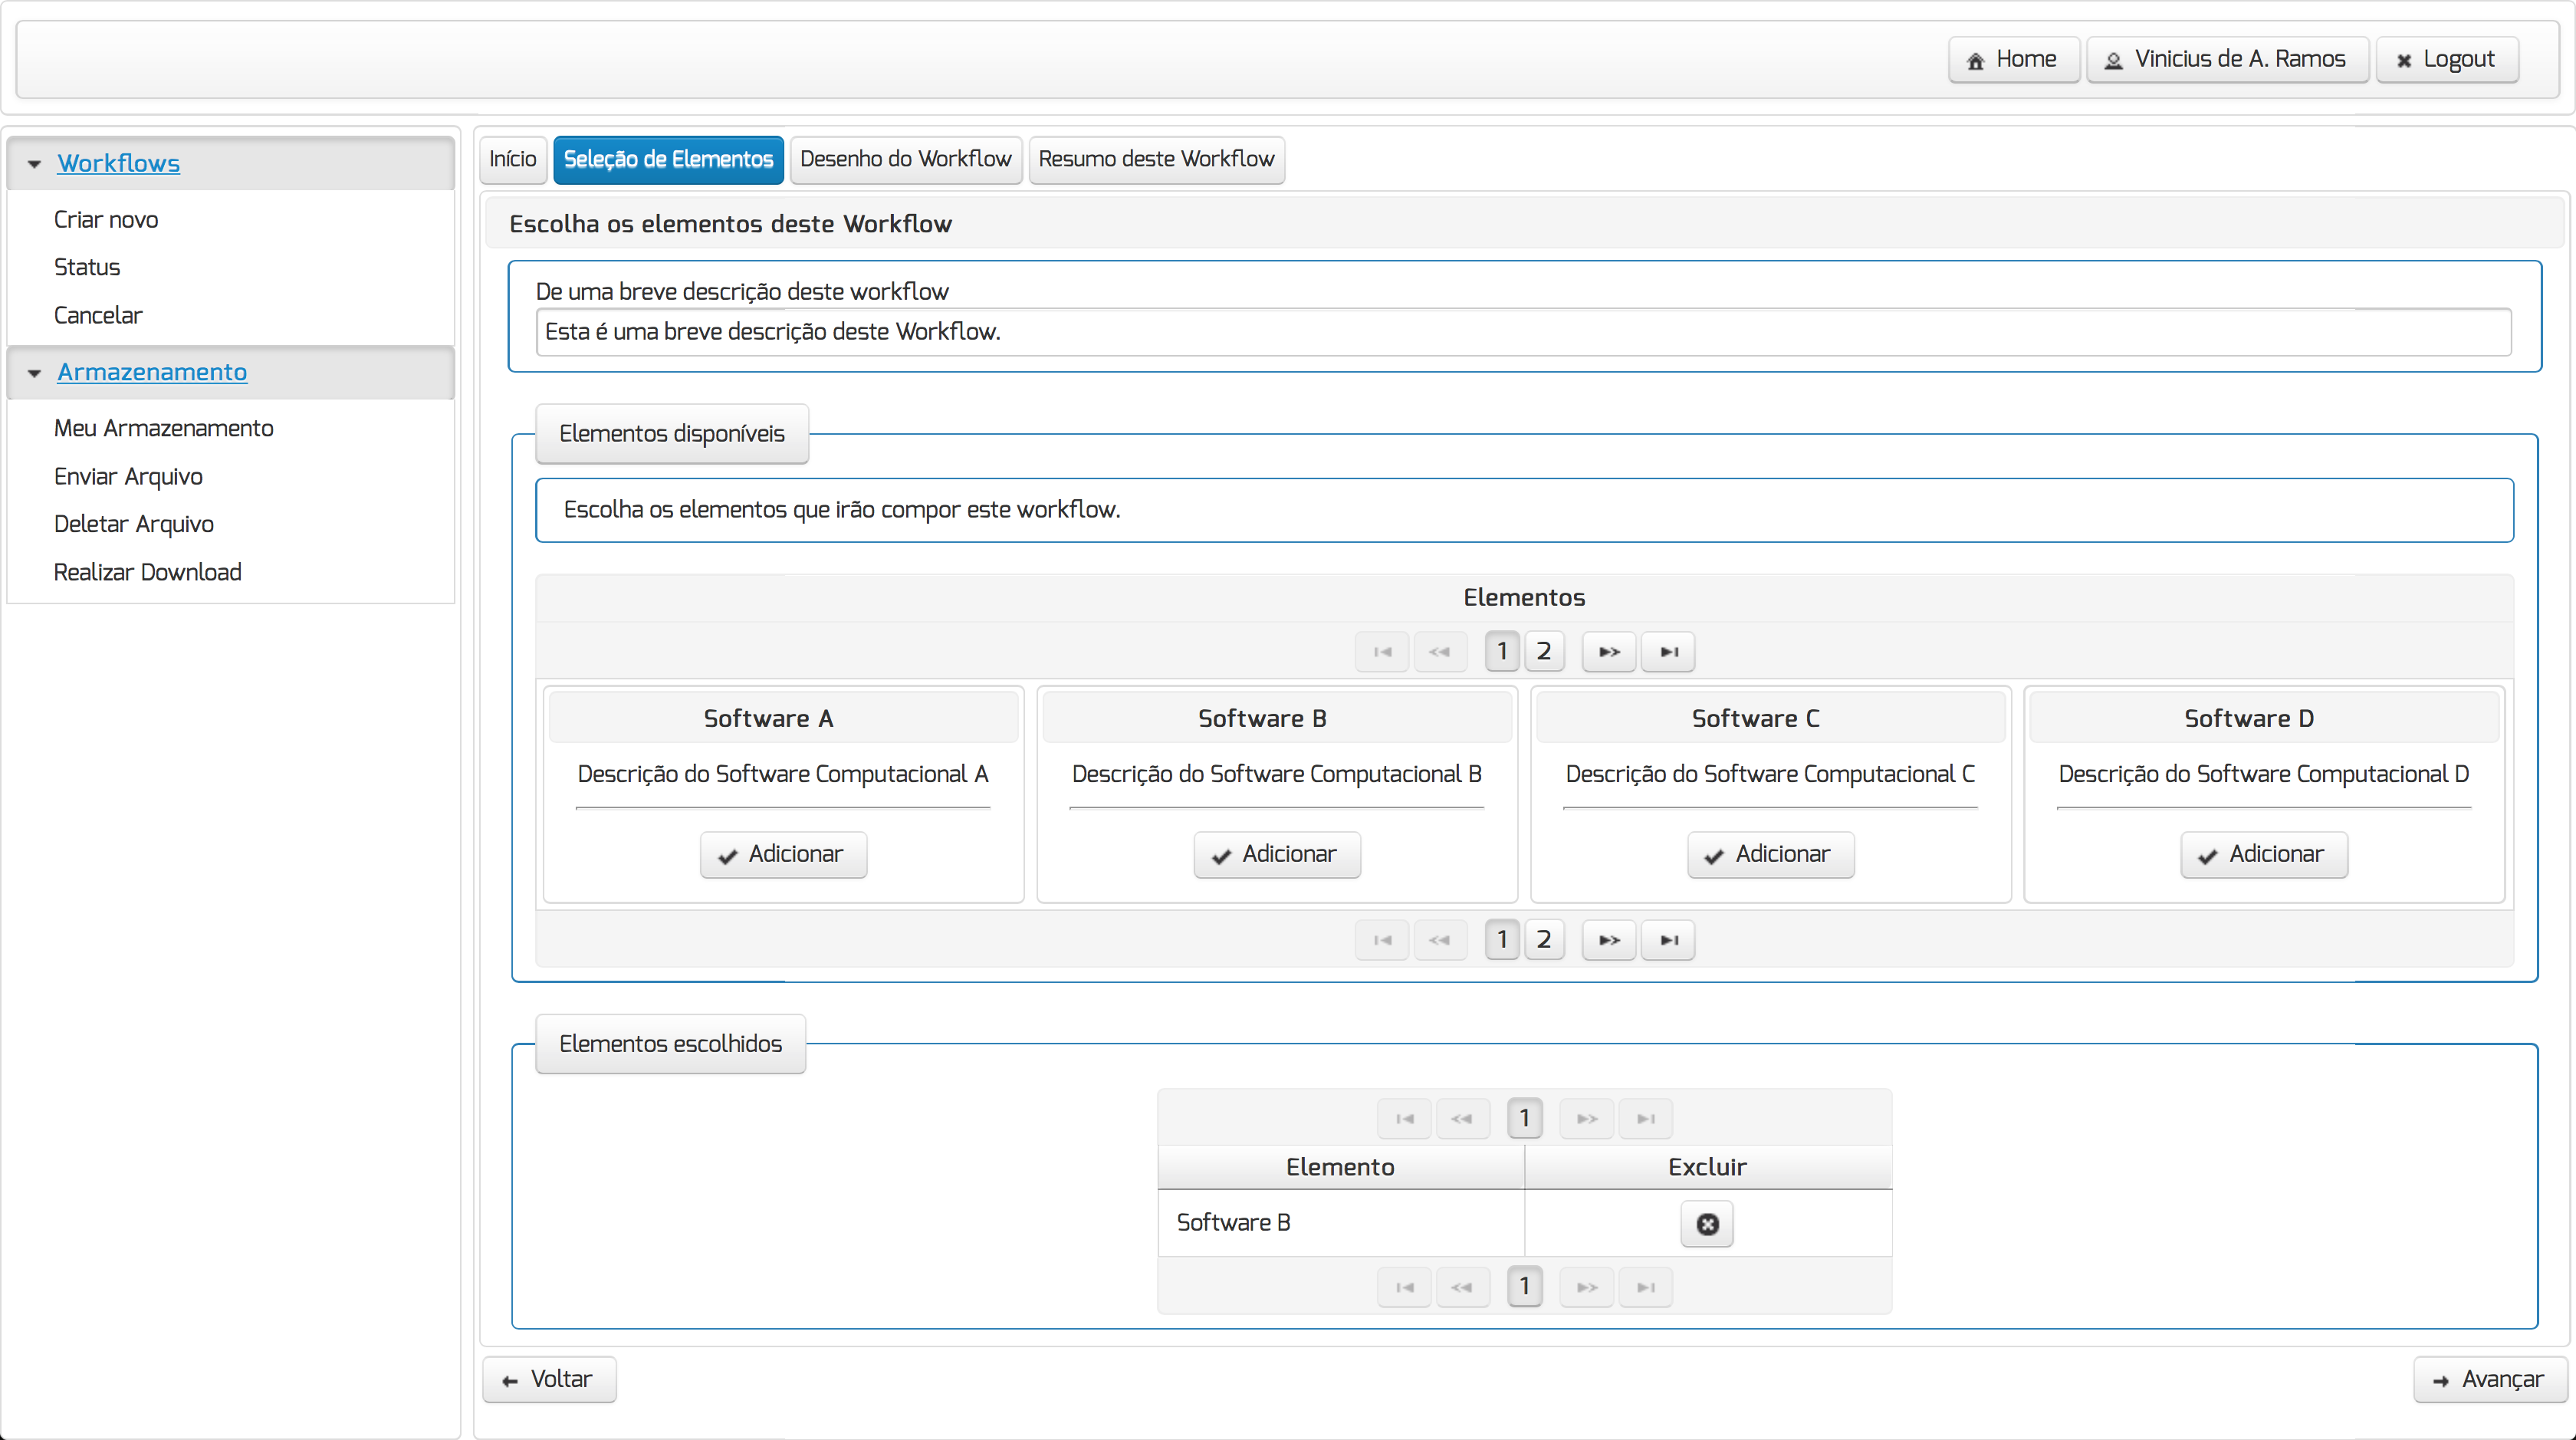
\includegraphics[scale=0.265 ]{tela_selecao_elementos.png}
	\caption{Tela utilizada para selecionar elementos que irão compôr o \textit{workflow}.}
	\label{fig:tela_selecao_elementos}
\end{figure}

\noindent
\textbf{Tela de \textit{design} do \textit{workflow}} \\

\noindent
Com os elementos definidos na tela anterior (Figura \ref{fig:tela_selecao_elementos}), o usuário é redirecionado para a tela seguinte, passando para a fase de \textit{design} do \textit{workflow}. Nela, são apresentados os elementos escolhidos pelo usuário dispostos de maneira gráfica, conforme mostra a \ref{fig:tela_design_workflow}.

\begin{figure}[H]
	\centering
	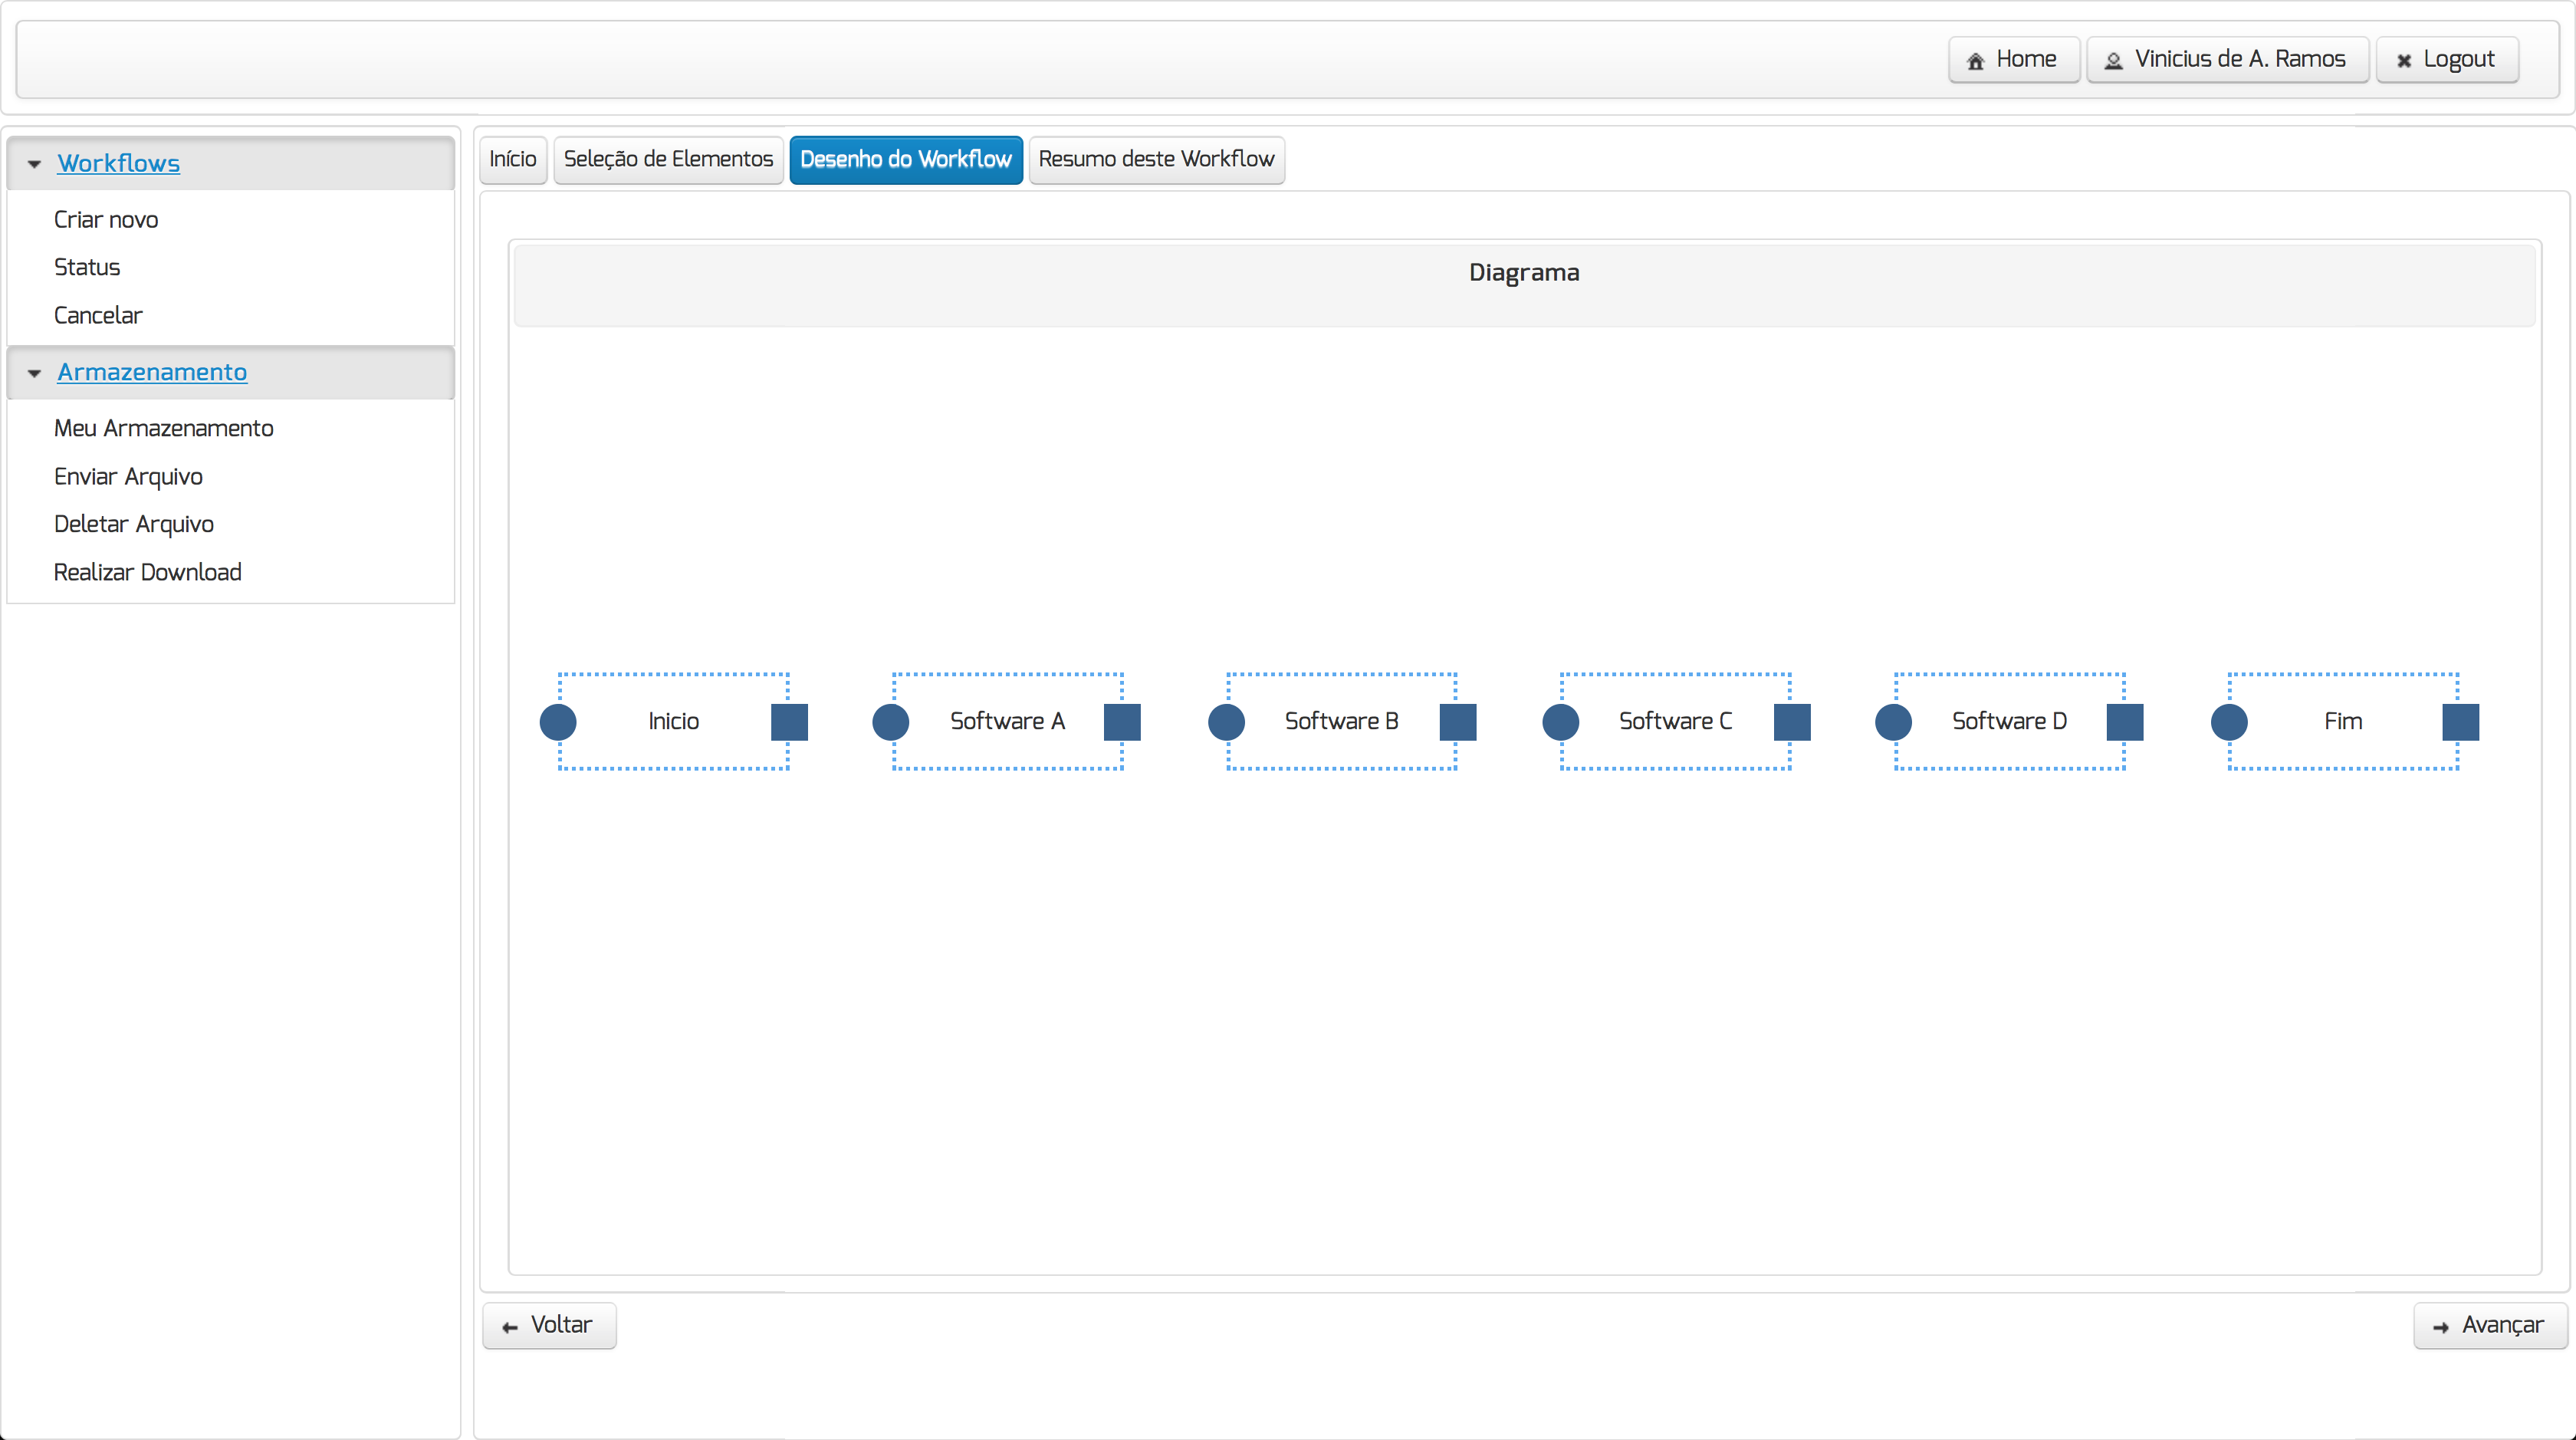
\includegraphics[scale=0.265 ]{tela_design_workflow.png}
	\caption{Nesta tela o usuário compõe o fluxo de seu \textit{workflow}.}
	\label{fig:tela_design_workflow}
\end{figure}

Com isso, o usuário pode definir as dependências de cada elemento, arrastando os pontos de ligação, definir suas entradas (arquivos enviados ou uma URL que contenha o caminho para realizar o download do arquivo para a plataforma BioNimbuZ), definir os parâmetros de execução (como argumentos daquele componente) ou apenas sinalizar que a entrada de um determinado elemento será a saída de outro. Para isso, ao se conectar dois elementos, é mostrada uma caixa de diálogo pedindo estes dados (Figura 5.9).

\begin{figure}[H]
	\centering
	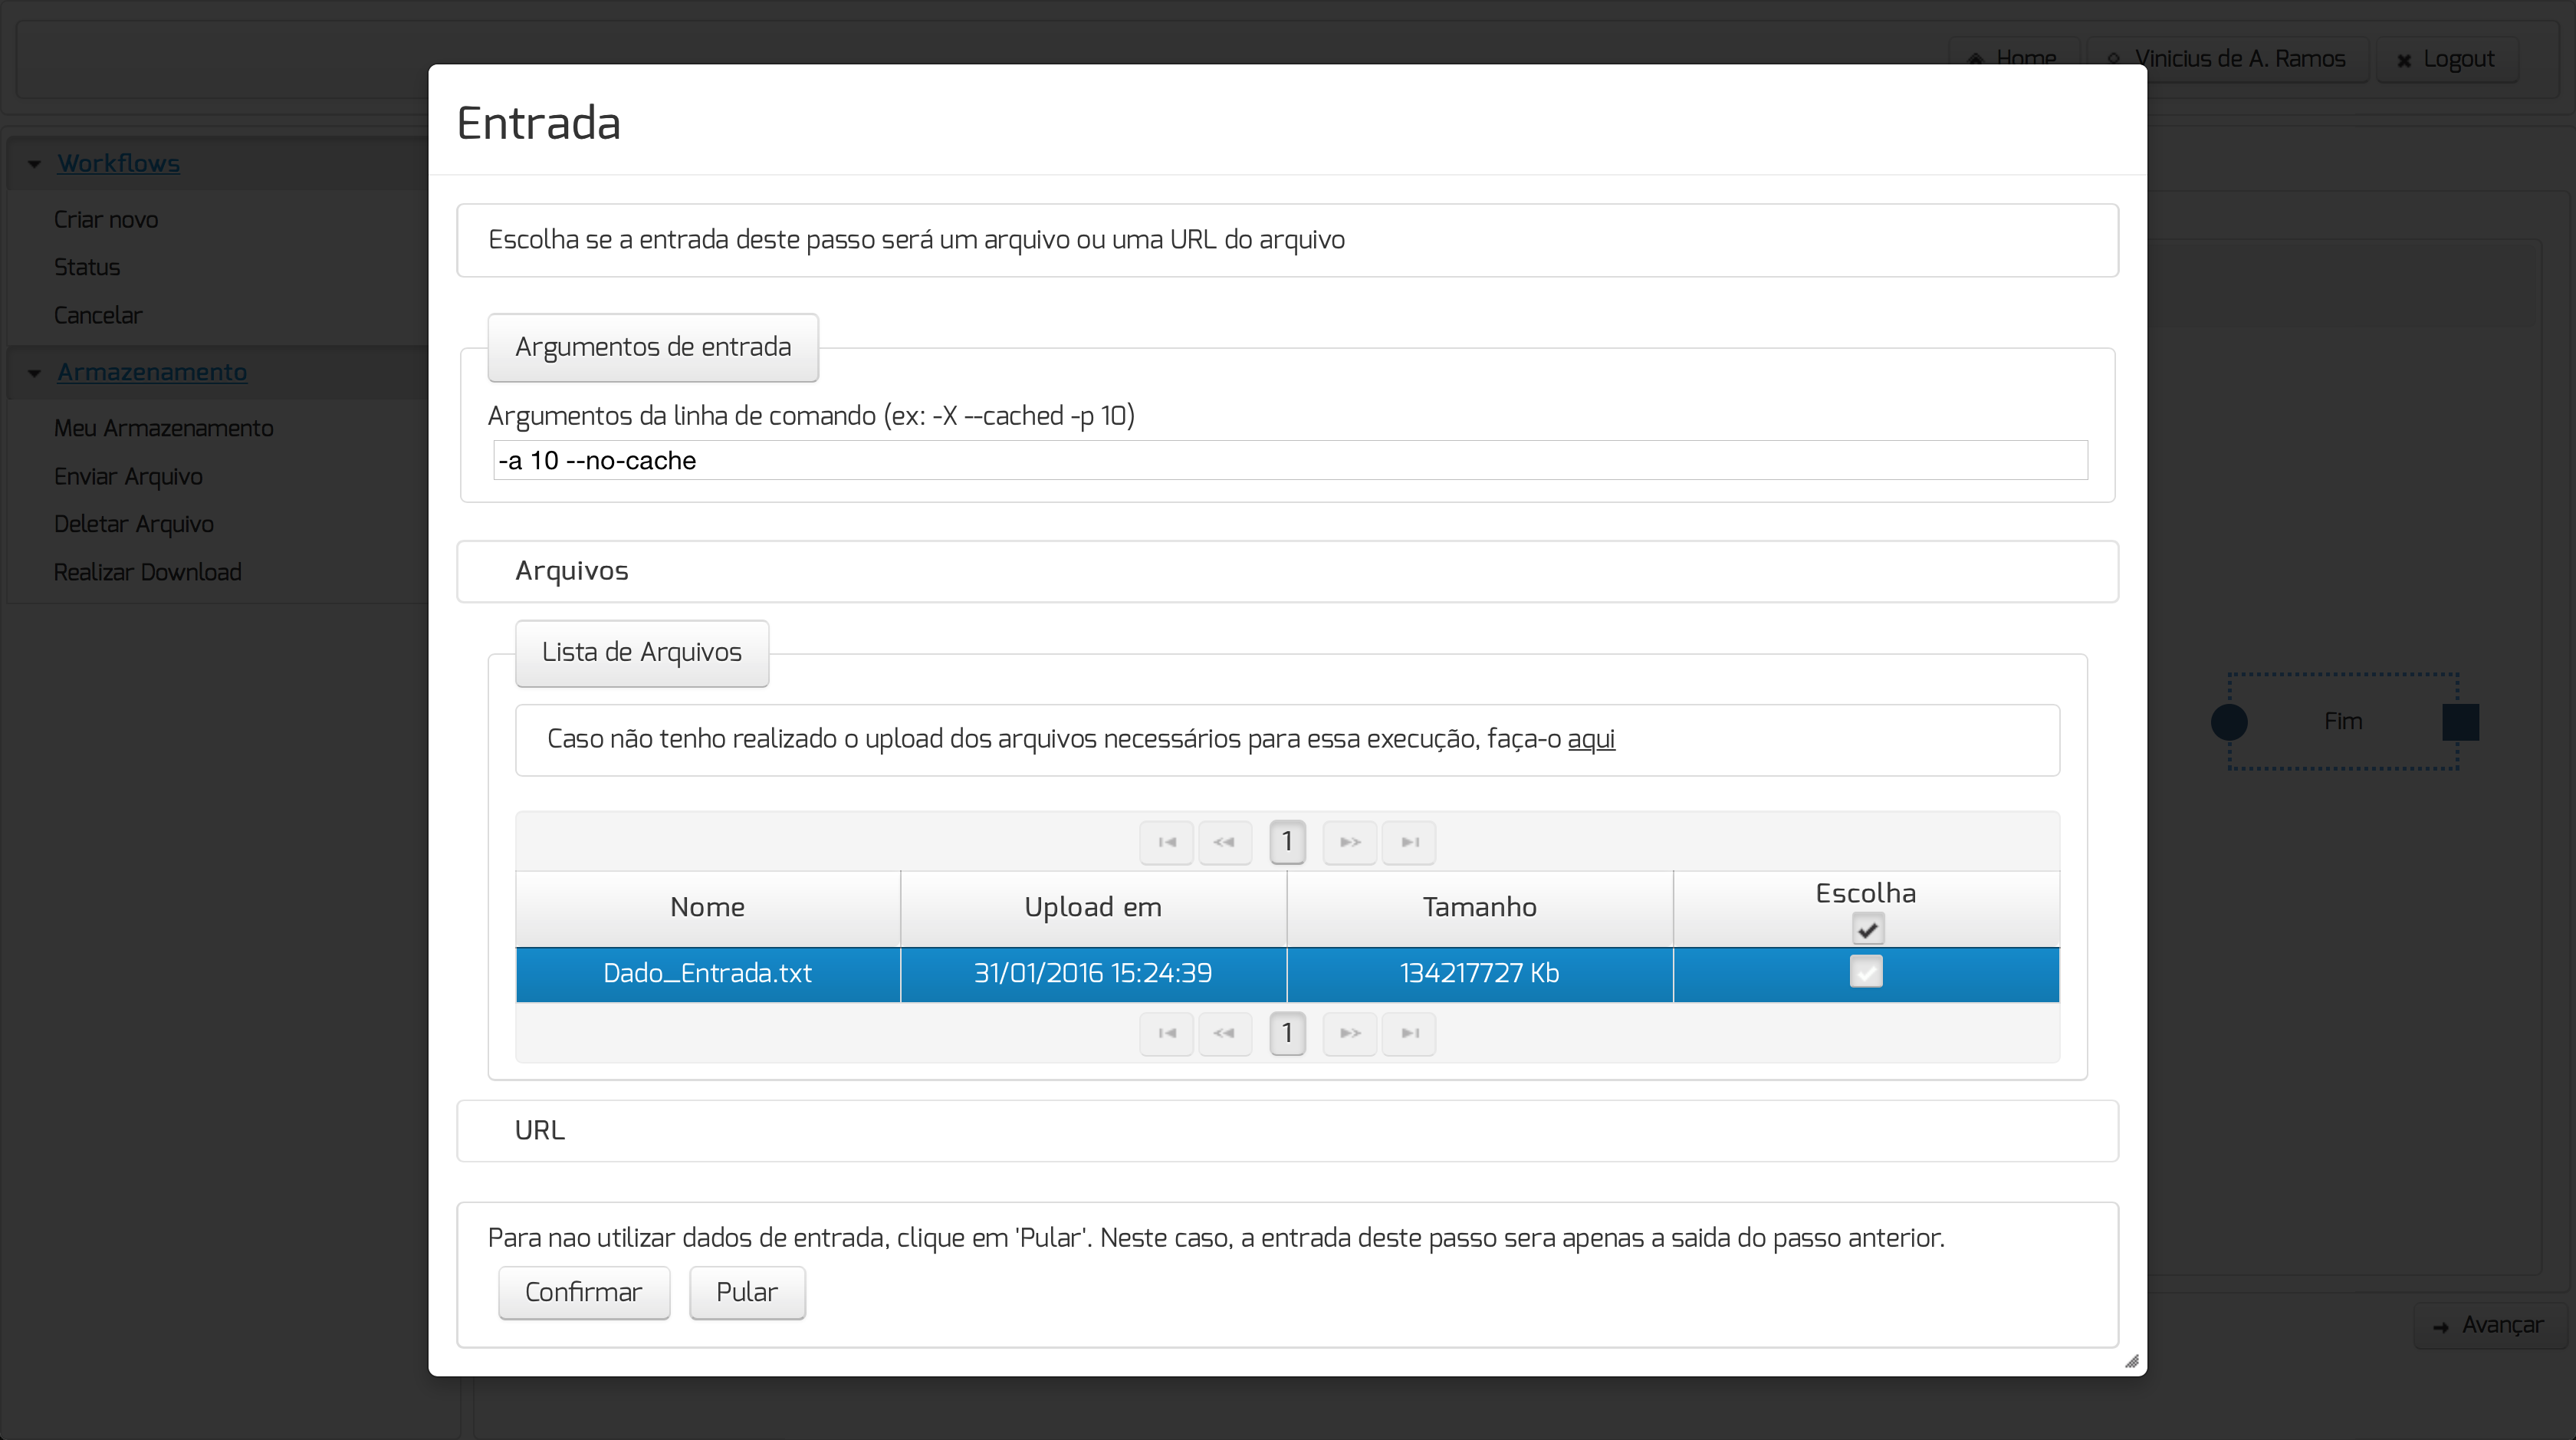
\includegraphics[scale=0.265 ]{tela_definicao_entrada.png}
	\caption{Nesta tela o usuário define parâmetros de execução de um elemento do \textit{workflow}.}
	\label{fig:tela_definicao_entrada}
\end{figure}

\noindent
\textbf{Tela de Confirmação} \\

\noindent
Com todos os elementos escolhidos e com suas dependências (entrada, saída e parâmetros de execução) satisfeitas, é apresentada uma tela de confimação (Figura \ref{fig:tela_final_workflow}), em que o usuário pode confirmar os dados daquele \textit{workflow} e submetê-lo à execução, ou pode apenas realizar o \textit{download} do arquivo \textbf{\textit{.flow}} (representação do objeto Java contendo os dados de um \textit{workflow}). De posse deste arquivo, o usuário pode importá-lo em outro momento para, por exemplo, finalizá-lo, ou também pode compartilhar este arquivo com outros usuários do sistema, para que outros tenham acesso ao seu trabalho.

\begin{figure}[H]
	\centering
	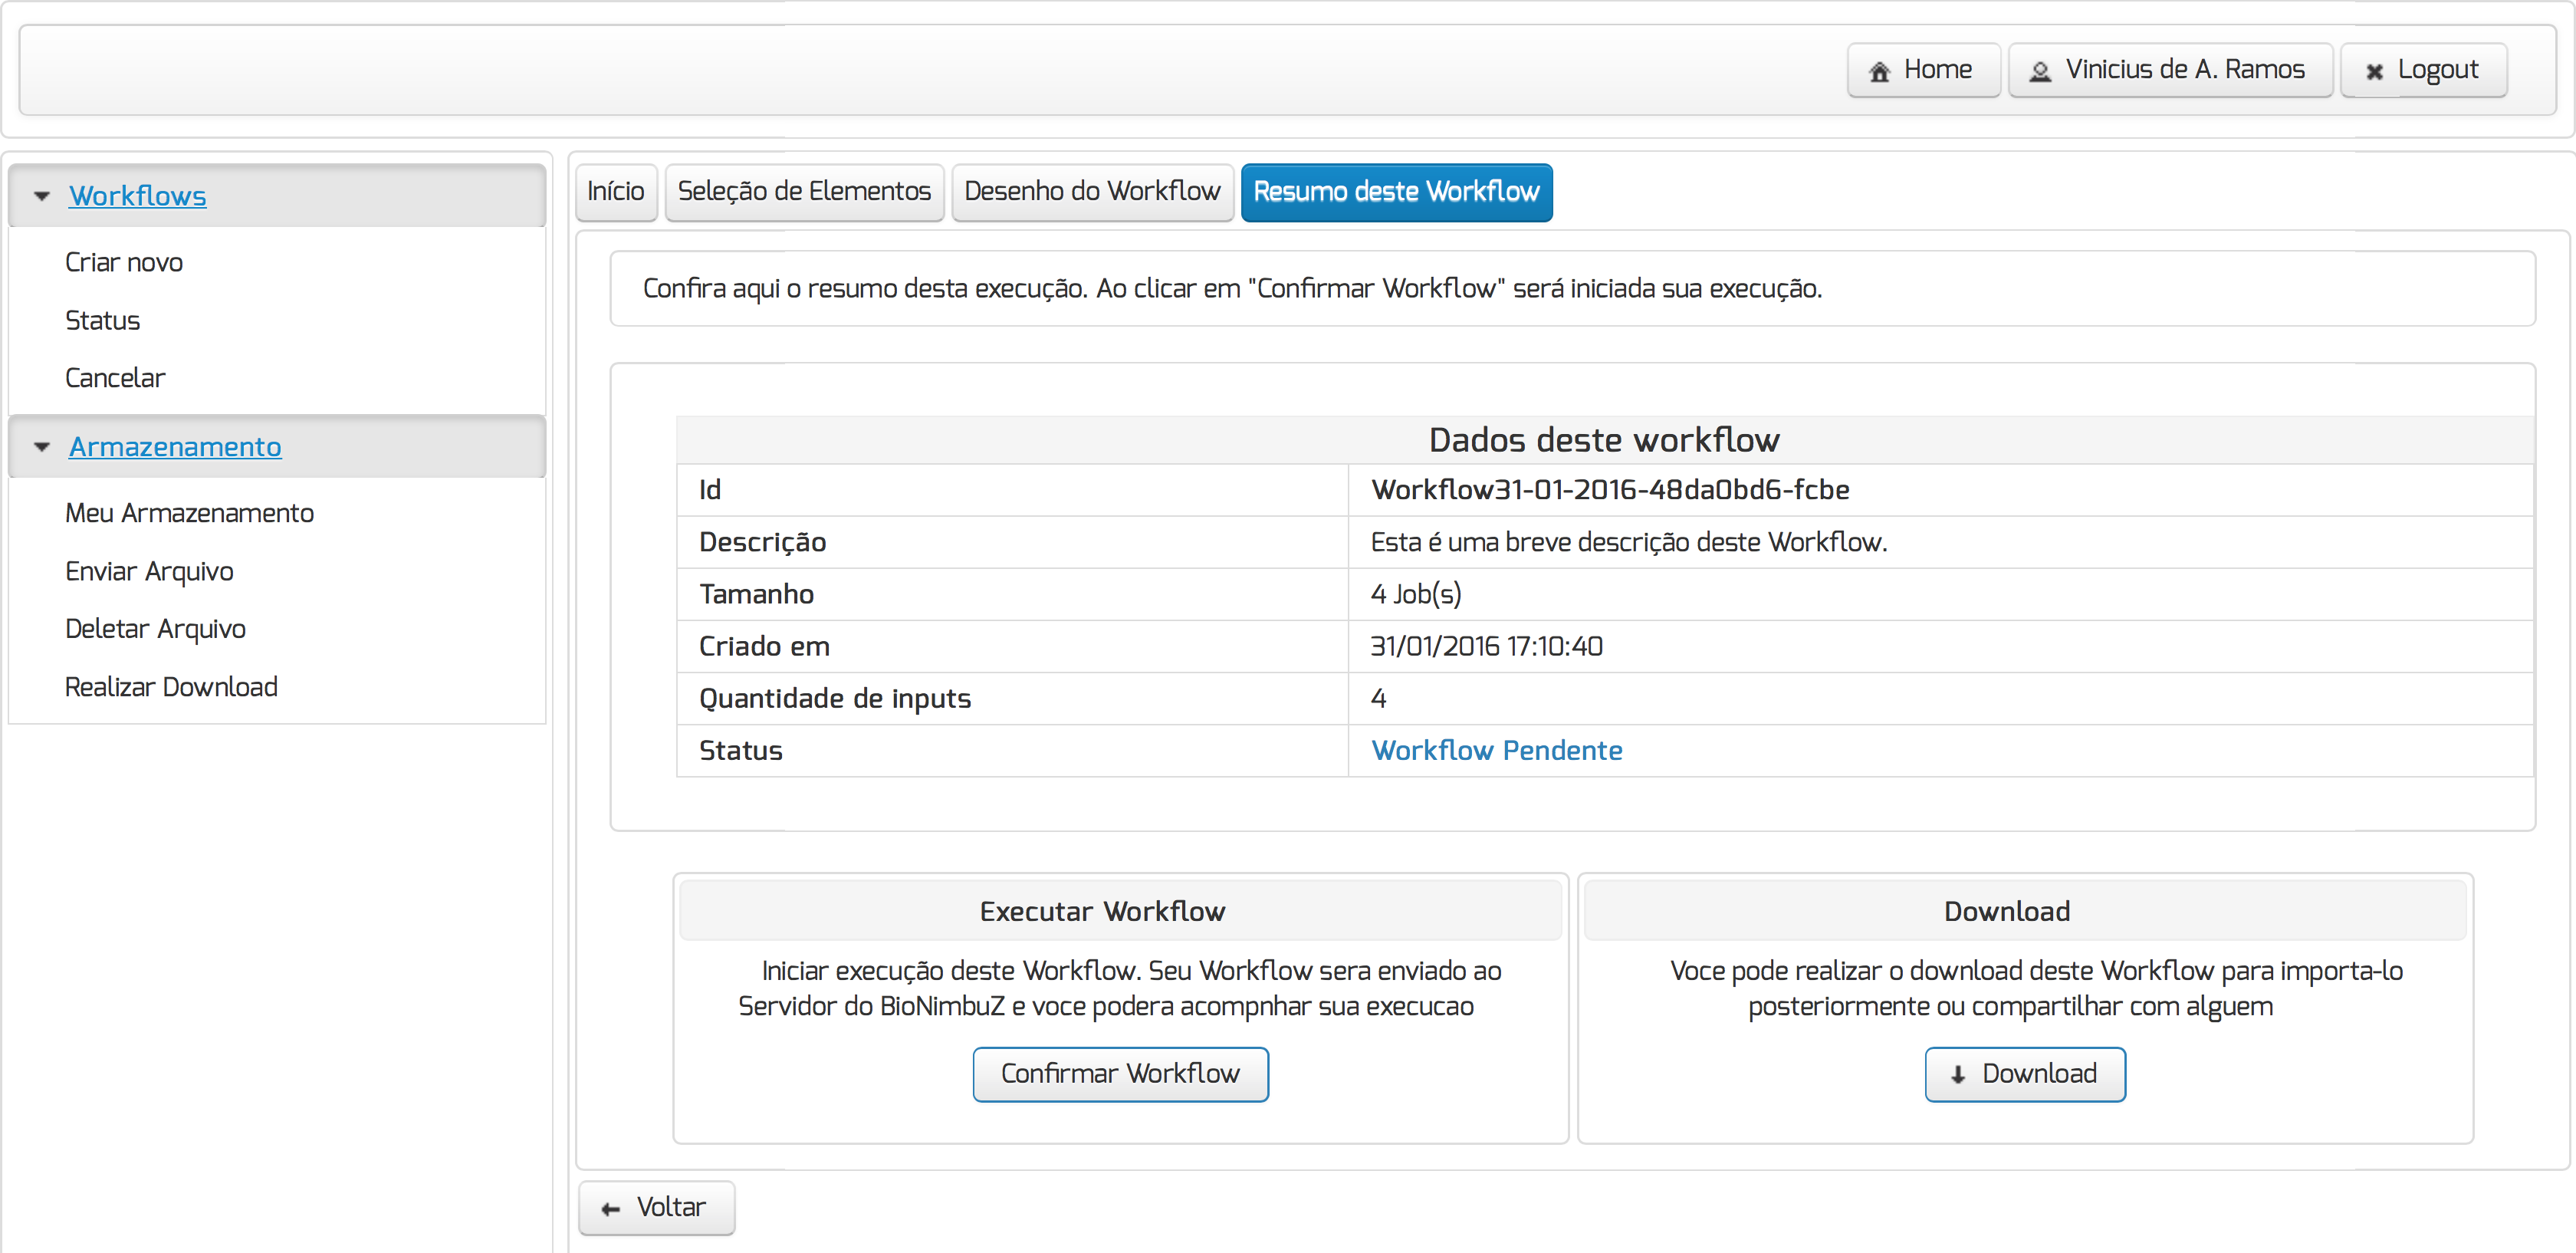
\includegraphics[scale=0.265 ]{tela_final_workflow.png}
	\caption{Tela final da composição do \textit{workflow}.}
	\label{fig:tela_final_workflow}
\end{figure}

\noindent
\textbf{Tela de \textit{status} do \textit{workflow}} \\

\noindent
A partir do momento que o usuário escolheu submeter o \textit{workflow} à plataforma BioNimbuZ, ele pode visualizar o estado de sua execução na tela de \textit{status}, apresentada na Figura \ref{tela_status_workflow}. 

\begin{figure}[H]
	\centering
	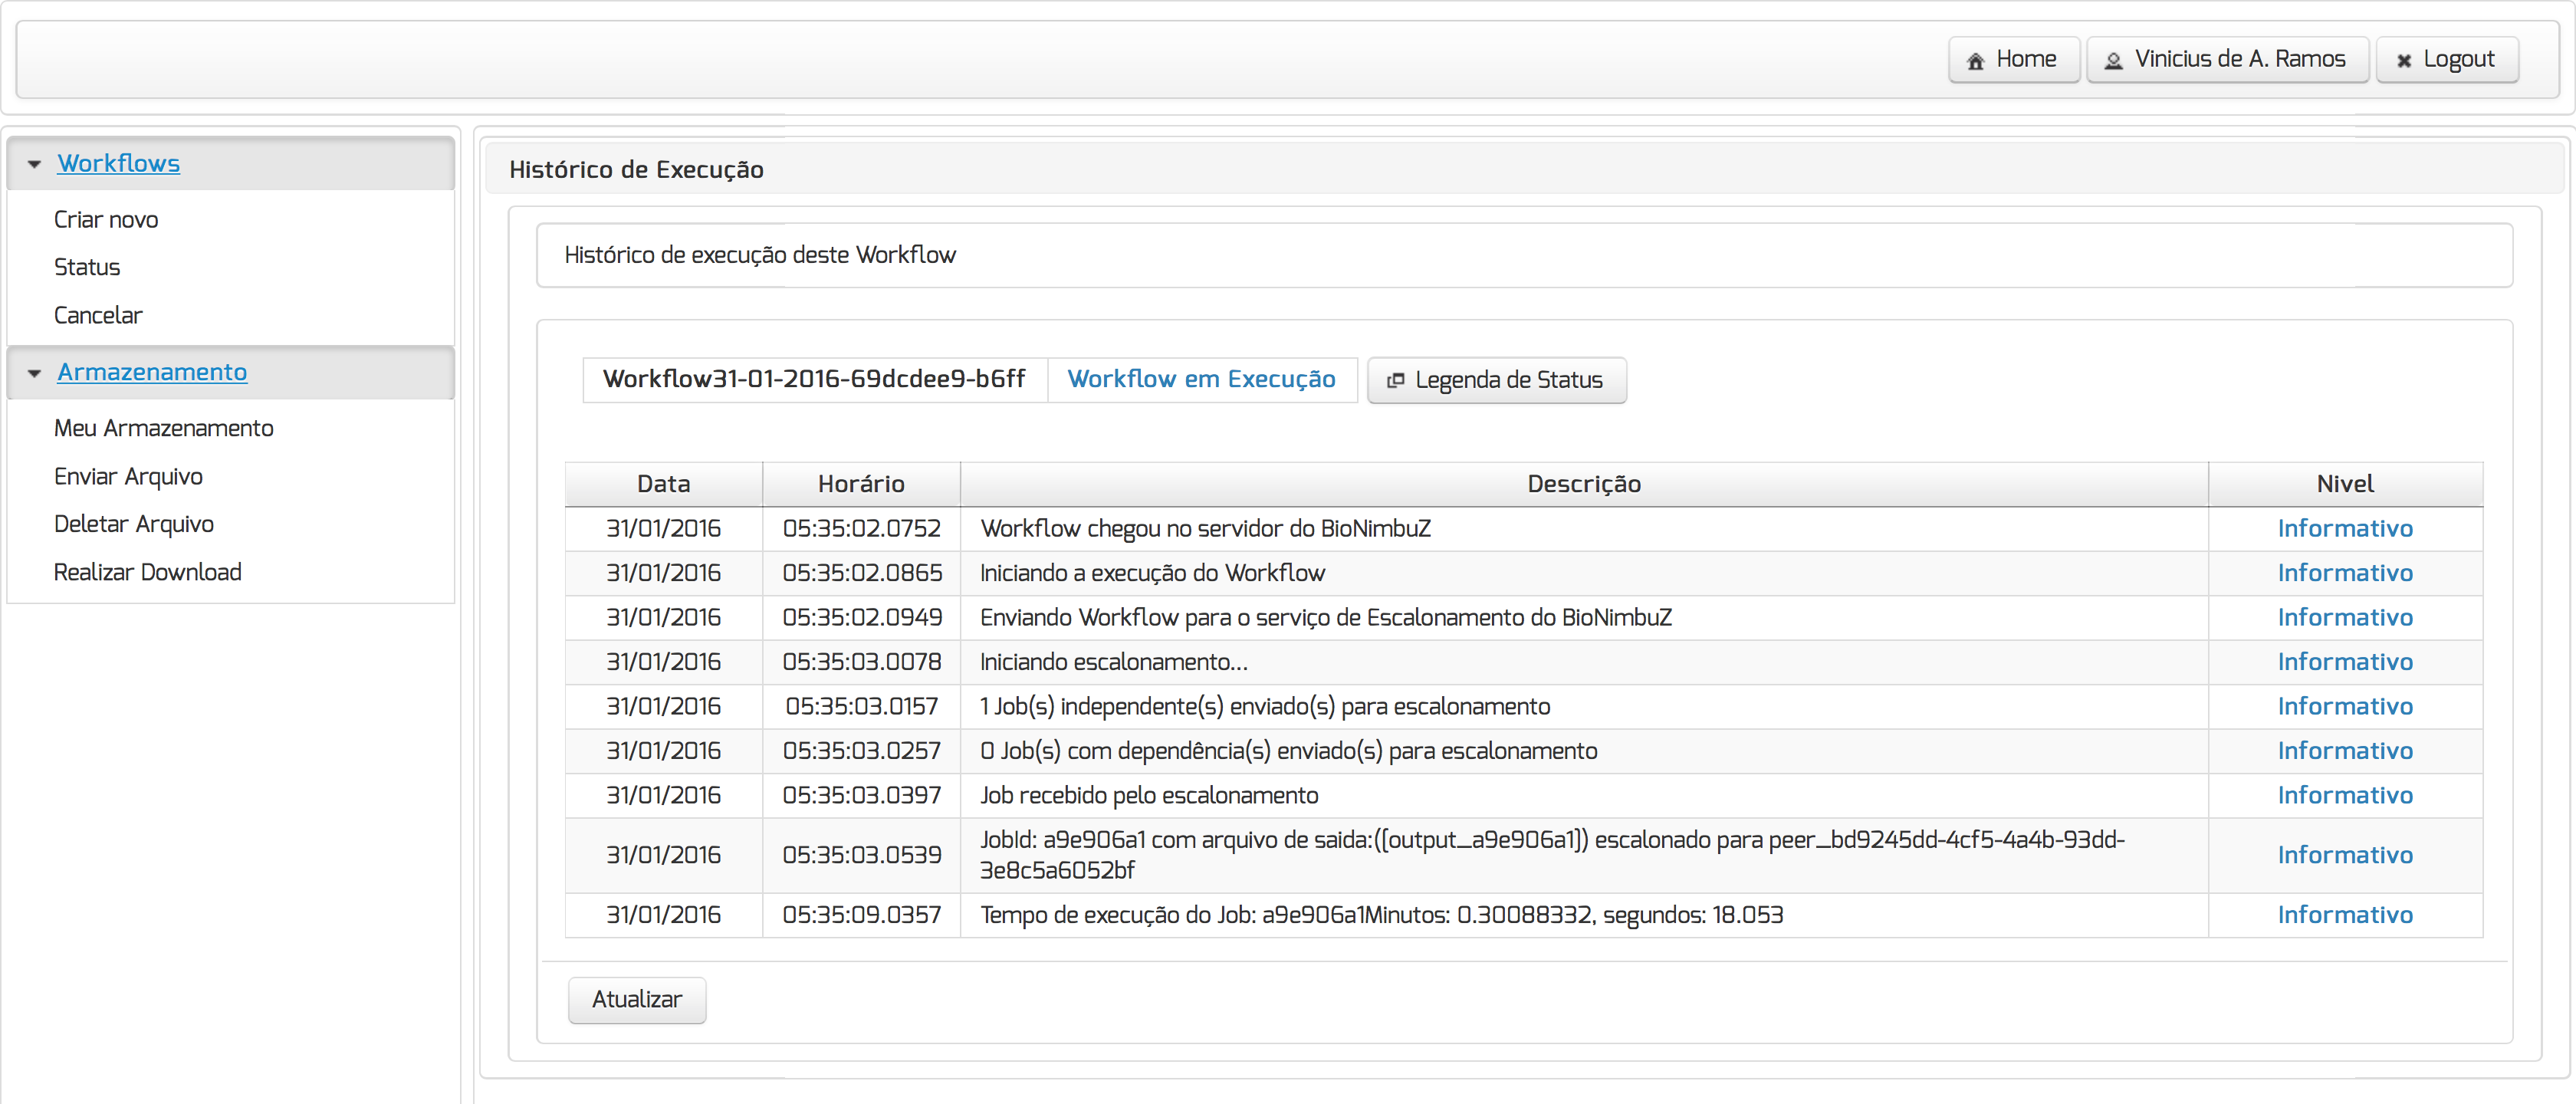
\includegraphics[scale=0.265 ]{tela_status_workflow.png}
	\caption{Tela final da composição do \textit{workflow}.}
	\label{fig:tela_status_workflow}
\end{figure}

Os possíveis estados de um \textit{workflow} estão retratados na Tabela \ref{tab:tabela_status_workflow}.


\begin{table}[H]
\centering
\resizebox{\textwidth}{!}{%
\begin{tabular}{||c|c|c||}
\hline
\large{\textbf{\textit{Status}}} & \large{\textbf{Nível}} & \large{\textbf{Descrição}} \\
\hline
\hline
\multicolumn{1}{||l|}{{\color[HTML]{7F8C8D} \textbf{\textit{Workflow} Pausado}}}                & \multicolumn{1}{l|}{\texttt{Informativo}} & \multicolumn{1}{l||}{Foi requisitada a pausa na execução do \textit{Workflow}.}               \\ 
\hline
\multicolumn{1}{||l|}{{\color[HTML]{2980B9} \textbf{\textit{Workflow} Pendente}}}               & \multicolumn{1}{l|}{\texttt{Informativo}} & \multicolumn{1}{l||}{Seu \textit{Workflow} está agurdando execução pelo BioNimbuZ.}           \\ 
\hline
\multicolumn{1}{||l|}{{\color[HTML]{2980B9} \textbf{\textit{Workflow} em Execução}}}            & \multicolumn{1}{l|}{\texttt{Informativo}} & \multicolumn{1}{l||}{O \textit{Workflow} está em plena execução.}                             \\ 
\hline
\multicolumn{1}{||l|}{{\color[HTML]{27AE60} \textbf{\textit{Workflow} Finalizado com Sucesso}}} & \multicolumn{1}{l|}{\texttt{Informativo}} & \multicolumn{1}{l||}{Seu \textit{Workflow} foi finalizado sem alertas e sem erros.}           \\ 
\hline
\multicolumn{1}{||l|}{{\color[HTML]{F39C12} \textbf{\textit{Workflow} Finalizado com Alertas}}} & \multicolumn{1}{l|}{\texttt{Alerta}}      & \multicolumn{1}{l||}{Alertas foram lançados durante a execução deste \textit{Workflow}.}      \\ 
\hline
\multicolumn{1}{||l|}{{\color[HTML]{C0392B} \textbf{\textit{Workflow} Finalizado com Erros}}}   & \multicolumn{1}{l|}{\texttt{Erro}}        & \multicolumn{1}{l||}{Erros nao permitiram que este \textit{Workflow} terminasse com sucesso.} \\ 
\hline
\multicolumn{1}{||l|}{{\color[HTML]{C0392B} \textbf{\textit{Workflow} Parado com Erros}}}       & \multicolumn{1}{l|}{\texttt{Erro}}        & \multicolumn{1}{l||}{Estado parcial com erros.}                                      \\
\hline
\end{tabular}
}
\caption{Estados possíveis de um \textit{Workflow}}
\label{tab:tabela_status_workflow}
\end{table}


\noindent
\textbf{Telas de \textit{upload} de arquivos e armazenamento} \\

\noindent
À fim de se compôr um \textit{workflow}, o usuário tem duas formas de lhe prover dados de entrada: utilizando uma \textit{URL} para passar o caminho de rede de onde se encontra o arquivo, para que dessa forma o núcleo do BioNimbuZ possa realizar o \textit{download} do mesmo, ou enviar arquivos para a plataforma do BioNimbuZ, a partir da tela mostrada na Figura \ref{fig:tela_upload}. 

\begin{figure}[H]
	\centering
	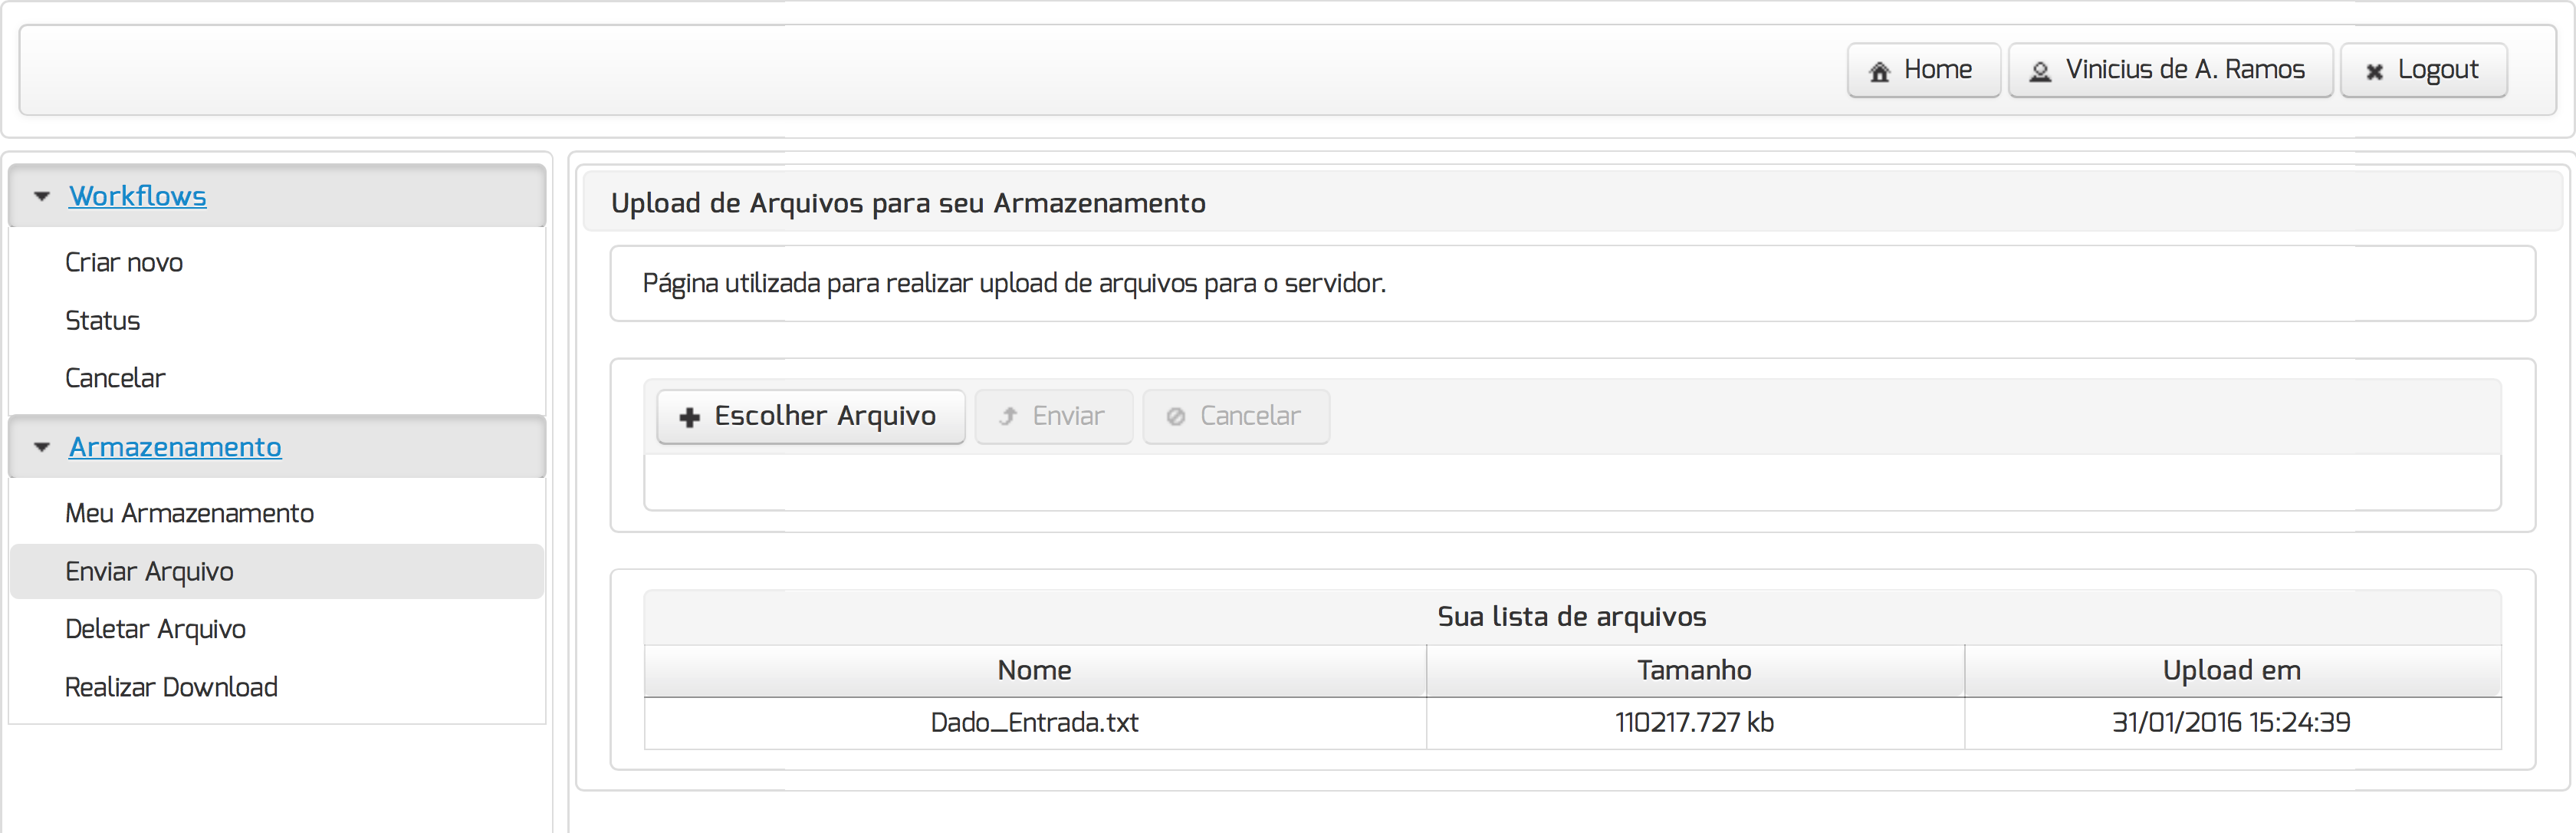
\includegraphics[scale=0.265 ]{tela_upload.png}
	\caption{Tela utilizada para realizar o \textit{upload} de arquivos.}
	\label{fig:tela_upload}
\end{figure}

Nesta implementação, foi definido um armazenamento máximo de 256 \textit{Megabytes} por usuário. Foi desenvolvida uma interface para que usuários possam ter controle de seu armazenamento, apresentada na Figura \ref{fig:tela_armazenamento}.

\begin{figure}[H]
	\centering
	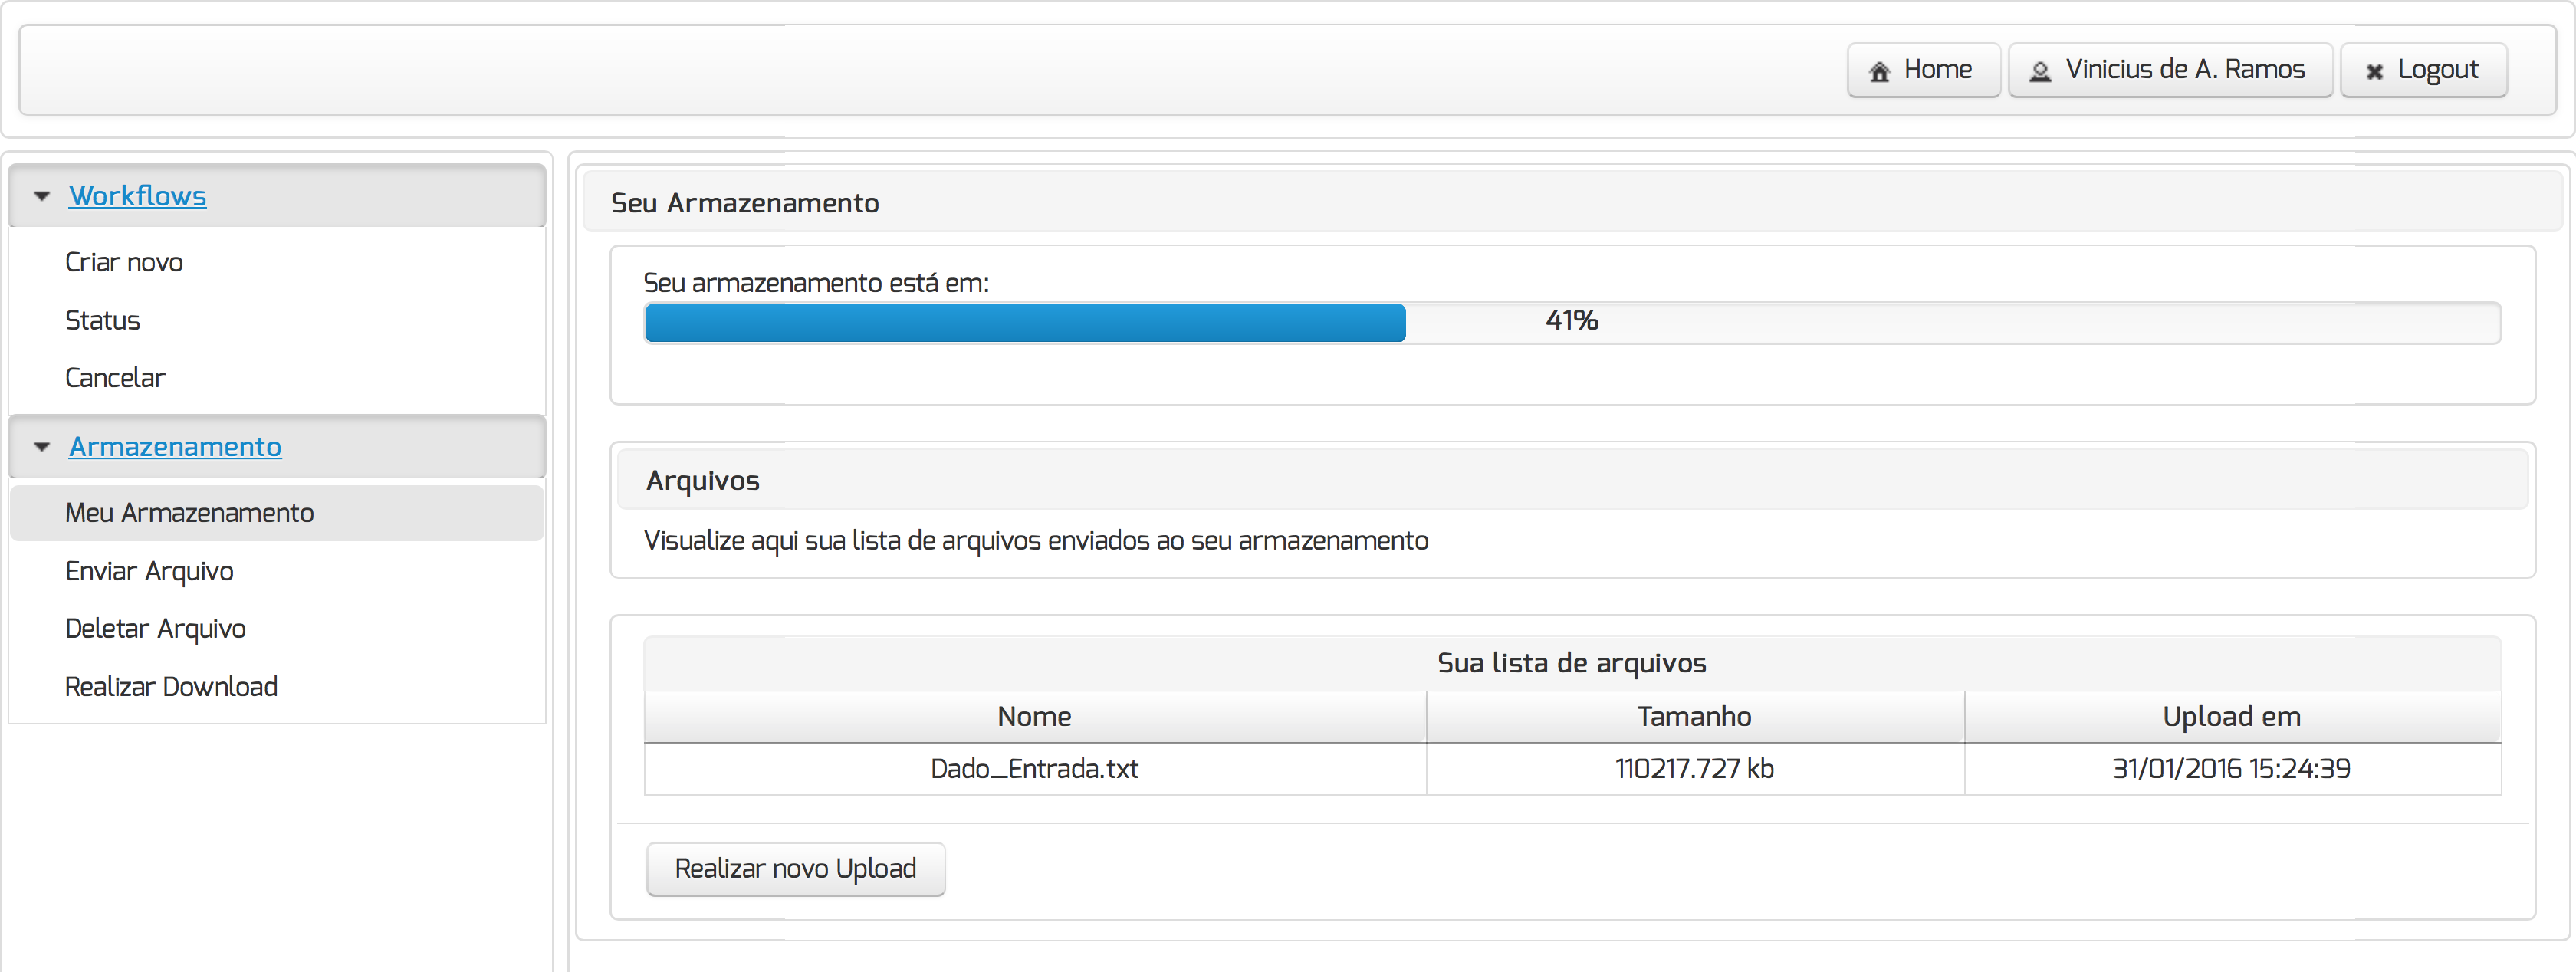
\includegraphics[scale=0.265]{tela_armazenamento.png}
	\caption{Nesta tela usuários controlam seu armazenamento e verificam sua porcentagem.}
	\label{fig:tela_armazenamento}
\end{figure}

Desta forma, as telas apresentadas compõem a camada de visualização do Modelo \textit{MVC}. A Seção 

A Seção \ref{cap5sec3subsec2} trata da Camada de Controle, a qual também compõe o Modelo \textit{MVC}.

\subsection{Camada de Controle} \label{cap5sec3subsec2}

Conforme o que foi exposto previamente, a camada de controle tem a responsabilidade de interpretar os dados enviados pelo usuário, a partir da camada de visualização (que neste projeto foi desenvolvida a partir de páginas \textit{HTML}), sinalizando ao sistema o que aqueles comandos representam.

Assim, foram desenvolvidas classes Java controladoras para tratar as requisições disparadas nas páginas \textit{web} de forma que houvesse uma ligação entre as classes Java e suas respectiva páginas \textit{HTML}. Essa correspondência é mostrada na Tabela \ref{tab:tabela_clases_paginas} e descrita a seguir:

\begin{table}[H]
\centering
\resizebox{\textwidth}{!}{%
\begin{tabular}{||c|c||}
\hline
\textbf{Classe Java} & \textbf{Página relacionada}  \\
\hline
\hline
\multicolumn{1}{||l|}{\code{SessionBean}}				& \multicolumn{1}{l||}{Página de \textit{login}} \\ 
\hline
\multicolumn{1}{||l|}{\code{SignUpBean}}				& \multicolumn{1}{l||}{Página de cadastro de novos usuários} \\
\hline
\multicolumn{1}{||l|}{\code{FileUploadBean}}			& \multicolumn{1}{l||}{Página relativa à \textit{upload} de arquivos} \\  
\hline
\multicolumn{1}{||l|}{\code{DeleteFileBean}} 			& \multicolumn{1}{l||}{Página de deleção de arquivos do usuário} \\ 
\hline
\multicolumn{1}{||l|}{\code{WorkflowComposerBean}} 	& \multicolumn{1}{l||}{Página de composição, \textit{design} e submissão de \textit{workflows}}      \\ 
\hline
\multicolumn{1}{||l|}{\code{WorkflowStatusBean}}		& \multicolumn{1}{l||}{Página para visualização do \textit{status} dos \textit{workflows} gerenciados pelo usuário}        \\ 
\hline
\multicolumn{1}{||l|}{\code{WorkflowHistoryBean}}		& \multicolumn{1}{l||}{Contém o histórico de execução de um determinado \textit{workflow}}        \\
\hline
\end{tabular}
}
\caption{Relação entre classes Java e páginas \textit{HTML}.}
\label{tab:tabela_clases_paginas}
\end{table}

\begin{itemize}
	\item \textbf{\texttt{SessionBean}:} Esta classe tem como função principal realizar ações relacionadas à sessão do usuário no sistema, como por exemplo executar o \textit{login} e o \textit{logout}. Também deve manter as informações acerca do usuário (dados pessoais, lista de arquivos, lista de \textit{workflows} submetidos, etc) para consulta por outros componentes do sistema, funcionando, portanto, como um repositório de dados de usuários;
	\item \textbf{\texttt{SignUpBean}:} Controla o fluxo do sistema quando um usuário deseja se cadastrar na plataforma, isto é, verifica se o usuário já foi cadastrado previamente, e, em caso negativo, realiza sua inclusão, persistindo-o no banco de dados;
	\item \textbf{\texttt{FileUploadBean}:} Responsável por enviar os arquivos dos usuários à plataforma BioNimbuZ. Também realiza o tratamento do arquivo, verificando aspectos tais como: 
	\begin{enumerate}	
		\item \textbf{Extensão:} Verifica se a extensão do arquivo satisfaz àquela esperada pelo sistema;
		\item \textbf{Tamanho:} Certifica-se de que o tamanho do arquivo enviado não ultrapassa o limite estipulado;
		\item \textbf{Nome de Arquivo:} Verifica se aquele nome de arquivo já não foi previamente enviado ao sistema.
	\end{enumerate}		
	\item \textbf{\texttt{DeleteFileBean}:} Sua função é deletar um arquivo de usuário, enviando a requisição de exclusão para o núcleo do BioNimbuZ e mostrando o resultado ao usuário (arquivo excluído ou erro no processamento);
	\item \textbf{\texttt{WorkflowComposerBean}:} Essa classe é a principal classe do sistema gerenciador de \textit{workflows} desenvolvido. Ela controla a página relativa à composição dos \textit{workflows}, fazendo toda verificação e validação dos dados de entradas, dos parâmetro de execução, do \textit{design} do \textit{workflow}, etc;
	\item \textbf{\texttt{WorkflowStatusBean}:} Requisita ao núcleo do BioNimbuZ o estado de um determinado \textit{workflow}, enviando, para isso, seu \texttt{ID}. Formata os dados de retorno, enviando-os à página \textit{HTML} para serem mostrados ao usuário;
	\item \textbf{\texttt{WorkflowHistoryBean}:} Envia requisições ao BioNimbuZ pedindo o passo-a-passo da execução de um dado \textit{workflow} (\textbf{\textit{log}}). Com este \textit{log}, o usuário pode, por exemplo, rastrear possíveis erros, propor melhorias ao seu fluxo ou analisar o passo-a-passo de execução de seu \textit{workflow}. Por fim esta classe formata a resposta enviada pelo núcleo e a disponibiliza à página \textit{web}.
\end{itemize}

A listagem acima demonstra a maioria das classes Java desenvolvidas com objetivo de controlar a camada de visualização, mas não todas. Outras classes auxiliares também foram implementadas, mas, por possuírem menor importância, não foram aqui citadas.

Dessa forma, essas classes realizam a função de controle do modelo \textit{MVC} que norteia o desenvolvimento da aplicação \textit{web}. A próxima Seção, \ref{cap5sec4}, trata da solução desenvolvida à fim de tratar o problema de comunicação entre a aplicação \textit{web} e o núcleo do BioNimbuZ.

% \subsection{Casos de Usos} \label{cap5sec3subsec1}

% \subsection{Fluxos das Ações} \label{cap5sec3subsec2}

\section{Camada de Comunicação} \label{cap5sec4}

Um dos requisitos da solução proposta era que os componentes de software compostos pela aplicação \textit{web} e pelo núcleo do BioNimbuZ fossem desenvolvidos de maneira distinta. Dessa forma, surgiu o problema de comunicação entre esses dois elementos.

Nesse contexto, a solução desenvolvida tem como base a comunicação utilizando-se \textit{webservices REST}(\textit{\textbf{RE}presentational \textbf{S}tate \textbf{T}ransfer}). \textit{REST} é definido como ''\textit{estilo de arquitetura para sistemas de hipermídia distribuídos, descrevendo os princípios de engenharia de software que guiam o  e as restrições de interação escolhidos para manter esses princípios, enquanto contrastando-as com as restrições de outros estilos arquiteturais.}'' \cite{rest}. Voltado para sistema baseados na Internet, tem sido amplamente utilizado na integração de sistemas, pois utiliza operações definidas no protocolo \textit{HTTP} (tais como \textit{PUT}, \textit{GET} e \textit{DELETE}). Assim, softwares que ''entendam'' o protocolo \textit{HTTP}, podem utilizar, geralmente, soluções baseadas em \textit{REST}.

Dessa forma, para possibilitar a troca de mensagens entre a aplicação \textit{web} e o núcleo do BioNimbuZ, foi necessário o desenvolvimento de três entidades principais: \textbf{Requisições} (\textit{requests}), \textbf{Respostas} (\textit{responses}) e \textbf{Ações} (\textit{actions}), com as seguintes responsabilidades:

\begin{itemize}
	\item \textbf{Ações:} Definem o comando à ser executado pelo núcleo, enviando-lhe uma requisição, à fim de se obter uma resposta com os dados requeridos;
	\item \textbf{Requisições:} De acordo com \cite{rest}, toda requisição feita à um servidor deve conter todo o conjunto de informações necessárias para sua completude, pois a comunicação não deve manter estado (\textit{stateless}). Assim, foram desenvolvidas requisições que contivéssem todos os dados necessários para a execução daquela Ação requisitada pela aplicação \textit{web};
	\item \textbf{Respostas:}
\end{itemize}


\section{Alterações realizadas no Núcleo do BioNimbuZ} \label{cap5sec5}
    
Compreende os serviços providos atualmente pelo BioNimbuz (como serviço de armazenamento, escalonamento, descobrimento) acrescido do código necessário para executar os comandos e requisições vindos da parte Cliente. Também deverá implementar métodos de acesso à bancos de dados relacionais, pois deverá persistir os dados trocados entre a aplicação Cliente e o Servidor do BioNimbuZ (entidades como Usuário, Workflow e Arquivo).

%Descrever a arquitetura do BioNimbuZ (Linha de comando, módulos, provedores, camadas...)
%-	Demonstrar o funcionamento anterior (linha de comando) e propor uma nova interface que dê %suporte ao desenvolvimento do novo módulo controlador de Jobs.
%-	Propor uma nova arquitetura baseada em aplicação WEB e comunicação com o núcleo via %webservices (Protocolo de troca de mensagens, tratamento de erros, ** solução de envio de %arquivos **).
%-	Propor uma nova política de upload de arquivos baseado em paralelização.
%-	Descrever as mudanças propostas (Protocolo de comunicação via REST, nova interface, %gerenciamento da execução de Jobs, nova política de envio de arquivos...)
%-	Explicar os temas: webservices, REST, servidor de aplicação, aplicação WEB, gerenciamento de %Jobs.
%-	Quais as vantagens e desvantagens das soluções propostas
%
%Descrever mudanças realizadas no BioNimbuZ
%-	Aplicação WEB
%-	Protocolo de Comunicação via WebServices
%-	Interface de Comunicação "Aplicação - Núcleo"
%-	Gerenciador de Estado dos Jobs (JobController)



